\documentclass[]{book}
\usepackage{lmodern}
\usepackage{amssymb,amsmath}
\usepackage{ifxetex,ifluatex}
\usepackage{fixltx2e} % provides \textsubscript
\ifnum 0\ifxetex 1\fi\ifluatex 1\fi=0 % if pdftex
  \usepackage[T1]{fontenc}
  \usepackage[utf8]{inputenc}
\else % if luatex or xelatex
  \ifxetex
    \usepackage{mathspec}
  \else
    \usepackage{fontspec}
  \fi
  \defaultfontfeatures{Ligatures=TeX,Scale=MatchLowercase}
\fi
% use upquote if available, for straight quotes in verbatim environments
\IfFileExists{upquote.sty}{\usepackage{upquote}}{}
% use microtype if available
\IfFileExists{microtype.sty}{%
\usepackage{microtype}
\UseMicrotypeSet[protrusion]{basicmath} % disable protrusion for tt fonts
}{}
\usepackage[margin=1in]{geometry}
\usepackage{hyperref}
\hypersetup{unicode=true,
            pdftitle={R로 배우는 기초통계},
            pdfauthor={한국생명공학연구원 김하성},
            pdfborder={0 0 0},
            breaklinks=true}
\urlstyle{same}  % don't use monospace font for urls
\usepackage{natbib}
\bibliographystyle{apalike}
\usepackage{color}
\usepackage{fancyvrb}
\newcommand{\VerbBar}{|}
\newcommand{\VERB}{\Verb[commandchars=\\\{\}]}
\DefineVerbatimEnvironment{Highlighting}{Verbatim}{commandchars=\\\{\}}
% Add ',fontsize=\small' for more characters per line
\usepackage{framed}
\definecolor{shadecolor}{RGB}{248,248,248}
\newenvironment{Shaded}{\begin{snugshade}}{\end{snugshade}}
\newcommand{\KeywordTok}[1]{\textcolor[rgb]{0.13,0.29,0.53}{\textbf{#1}}}
\newcommand{\DataTypeTok}[1]{\textcolor[rgb]{0.13,0.29,0.53}{#1}}
\newcommand{\DecValTok}[1]{\textcolor[rgb]{0.00,0.00,0.81}{#1}}
\newcommand{\BaseNTok}[1]{\textcolor[rgb]{0.00,0.00,0.81}{#1}}
\newcommand{\FloatTok}[1]{\textcolor[rgb]{0.00,0.00,0.81}{#1}}
\newcommand{\ConstantTok}[1]{\textcolor[rgb]{0.00,0.00,0.00}{#1}}
\newcommand{\CharTok}[1]{\textcolor[rgb]{0.31,0.60,0.02}{#1}}
\newcommand{\SpecialCharTok}[1]{\textcolor[rgb]{0.00,0.00,0.00}{#1}}
\newcommand{\StringTok}[1]{\textcolor[rgb]{0.31,0.60,0.02}{#1}}
\newcommand{\VerbatimStringTok}[1]{\textcolor[rgb]{0.31,0.60,0.02}{#1}}
\newcommand{\SpecialStringTok}[1]{\textcolor[rgb]{0.31,0.60,0.02}{#1}}
\newcommand{\ImportTok}[1]{#1}
\newcommand{\CommentTok}[1]{\textcolor[rgb]{0.56,0.35,0.01}{\textit{#1}}}
\newcommand{\DocumentationTok}[1]{\textcolor[rgb]{0.56,0.35,0.01}{\textbf{\textit{#1}}}}
\newcommand{\AnnotationTok}[1]{\textcolor[rgb]{0.56,0.35,0.01}{\textbf{\textit{#1}}}}
\newcommand{\CommentVarTok}[1]{\textcolor[rgb]{0.56,0.35,0.01}{\textbf{\textit{#1}}}}
\newcommand{\OtherTok}[1]{\textcolor[rgb]{0.56,0.35,0.01}{#1}}
\newcommand{\FunctionTok}[1]{\textcolor[rgb]{0.00,0.00,0.00}{#1}}
\newcommand{\VariableTok}[1]{\textcolor[rgb]{0.00,0.00,0.00}{#1}}
\newcommand{\ControlFlowTok}[1]{\textcolor[rgb]{0.13,0.29,0.53}{\textbf{#1}}}
\newcommand{\OperatorTok}[1]{\textcolor[rgb]{0.81,0.36,0.00}{\textbf{#1}}}
\newcommand{\BuiltInTok}[1]{#1}
\newcommand{\ExtensionTok}[1]{#1}
\newcommand{\PreprocessorTok}[1]{\textcolor[rgb]{0.56,0.35,0.01}{\textit{#1}}}
\newcommand{\AttributeTok}[1]{\textcolor[rgb]{0.77,0.63,0.00}{#1}}
\newcommand{\RegionMarkerTok}[1]{#1}
\newcommand{\InformationTok}[1]{\textcolor[rgb]{0.56,0.35,0.01}{\textbf{\textit{#1}}}}
\newcommand{\WarningTok}[1]{\textcolor[rgb]{0.56,0.35,0.01}{\textbf{\textit{#1}}}}
\newcommand{\AlertTok}[1]{\textcolor[rgb]{0.94,0.16,0.16}{#1}}
\newcommand{\ErrorTok}[1]{\textcolor[rgb]{0.64,0.00,0.00}{\textbf{#1}}}
\newcommand{\NormalTok}[1]{#1}
\usepackage{longtable,booktabs}
\usepackage{graphicx,grffile}
\makeatletter
\def\maxwidth{\ifdim\Gin@nat@width>\linewidth\linewidth\else\Gin@nat@width\fi}
\def\maxheight{\ifdim\Gin@nat@height>\textheight\textheight\else\Gin@nat@height\fi}
\makeatother
% Scale images if necessary, so that they will not overflow the page
% margins by default, and it is still possible to overwrite the defaults
% using explicit options in \includegraphics[width, height, ...]{}
\setkeys{Gin}{width=\maxwidth,height=\maxheight,keepaspectratio}
\IfFileExists{parskip.sty}{%
\usepackage{parskip}
}{% else
\setlength{\parindent}{0pt}
\setlength{\parskip}{6pt plus 2pt minus 1pt}
}
\setlength{\emergencystretch}{3em}  % prevent overfull lines
\providecommand{\tightlist}{%
  \setlength{\itemsep}{0pt}\setlength{\parskip}{0pt}}
\setcounter{secnumdepth}{5}
% Redefines (sub)paragraphs to behave more like sections
\ifx\paragraph\undefined\else
\let\oldparagraph\paragraph
\renewcommand{\paragraph}[1]{\oldparagraph{#1}\mbox{}}
\fi
\ifx\subparagraph\undefined\else
\let\oldsubparagraph\subparagraph
\renewcommand{\subparagraph}[1]{\oldsubparagraph{#1}\mbox{}}
\fi

%%% Use protect on footnotes to avoid problems with footnotes in titles
\let\rmarkdownfootnote\footnote%
\def\footnote{\protect\rmarkdownfootnote}

%%% Change title format to be more compact
\usepackage{titling}

% Create subtitle command for use in maketitle
\providecommand{\subtitle}[1]{
  \posttitle{
    \begin{center}\large#1\end{center}
    }
}

\setlength{\droptitle}{-2em}

  \title{R로 배우는 기초통계}
    \pretitle{\vspace{\droptitle}\centering\huge}
  \posttitle{\par}
    \author{한국생명공학연구원 김하성}
    \preauthor{\centering\large\emph}
  \postauthor{\par}
      \predate{\centering\large\emph}
  \postdate{\par}
    \date{2019-09-04}

\usepackage{booktabs}
\usepackage{amsthm}
\makeatletter
\def\thm@space@setup{%
  \thm@preskip=8pt plus 2pt minus 4pt
  \thm@postskip=\thm@preskip
}
\makeatother

\begin{document}
\maketitle

{
\setcounter{tocdepth}{1}
\tableofcontents
}
\hypertarget{introduction--}{%
\chapter{Introduction 강의 개요}\label{introduction--}}

\begin{itemize}
\tightlist
\item
  장소: 한국생명공학연구원 연구동 세미나실 1213호 (매주수요일 13:00\textasciitilde{}16:00)
\item
  강사: 한국생명공학연구원 바이오합성연구센터 김하성
\item
  연락처: 042-860-4372, \href{mailto:haseong@kribb.re.kr}{\nolinkurl{haseong@kribb.re.kr}} (생명연 연구동 1143)
\item
  강의site: \url{https://greendaygh.github.io/Rstat2019/}
\end{itemize}

\hypertarget{goal--}{%
\section{Goal 강의 목표}\label{goal--}}

\begin{itemize}
\tightlist
\item
  이공계열 대학원생이 보다 쉽게 통계 이론을 습득하고 활용하는 능력을 배양하는데 주요 목적이 있음. 특히 데이터 분석용 프로그래밍언어인 R을 기반으로 한 실습을 통하여 프로그래밍 기술 습득과 함께 데이터를 다루는 능력을 배움으로써 이공계 연구에 있어서 필수인 통계적 사고의 기초를 다지는데 그 목적이 있음.
\end{itemize}

\hypertarget{references--}{%
\section{References 참고 자료}\label{references--}}

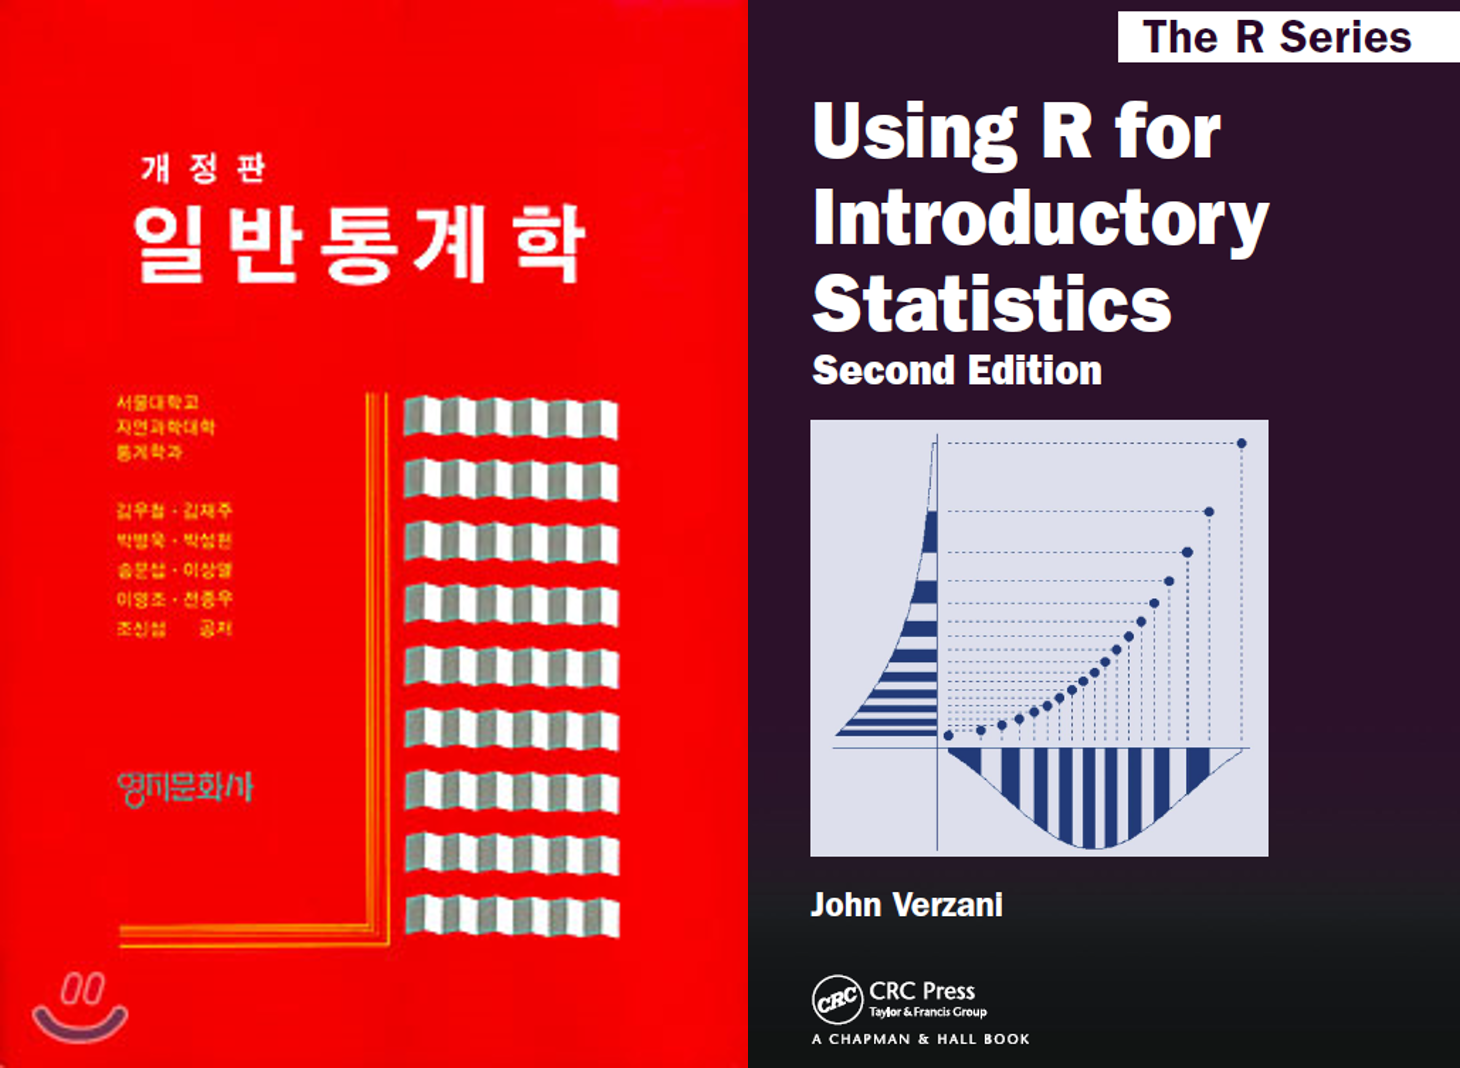
\includegraphics{images/01-15.PNG}

\begin{itemize}
\tightlist
\item
  Using R for Introductory Statistics by John Verzani

  \begin{itemize}
  \tightlist
  \item
    Free version of 1st Edition

    \begin{itemize}
    \tightlist
    \item
      \url{https://cran.r-project.org/doc/contrib/Verzani-SimpleR.pdf}
    \item
      \url{http://cbb.sjtu.edu.cn/~mywu/bi217/usingR.pdf}
    \end{itemize}
  \item
    Second edition

    \begin{itemize}
    \tightlist
    \item
      \url{https://www.crcpress.com/Using-R-for-Introductory-Statistics-Second-Edition/Verzani/p/book/9781466590731}
    \end{itemize}
  \end{itemize}
\item
  R for Data Science (\url{https://r4ds.had.co.nz}, \url{https://github.com/hadley})
\item
  \url{https://resources.rstudio.com/}
\item
  일반통계학 (영지문화사, 김우철 외)
\end{itemize}

\hypertarget{evaluation---}{%
\section{Evaluation 평가 세부 항목}\label{evaluation---}}

\begin{itemize}
\tightlist
\item
  출석 50\% / 과제 50\% / 80점 이상 S, 80점 미만 U 부여
\end{itemize}

\hypertarget{schedule--}{%
\section{Schedule 강의 계획}\label{schedule--}}

\begin{itemize}
\item
  1주차- R basics / introduction of data
\item
  2주차 - Univariate data -- Summary statistics 일변량자료 (범주형, 수치형, 분포)
\item
  3주차 - Bivariate data -- Correlation / Independence 이변량자료 (자료비교, 수치자료의 관계, 단순선형회귀)
\item
  4주차 - Multivariate data -- R data structure 다변량자료 (다변량, R자료형, R그래픽)
\item
  5주차 - Populations -- Families of distributions 모집단과 분포
\item
  6주차 - Sampling -- Distribution and CLT 시뮬레이션, 샘플링
\item
  7주차 - Statistical inference 통계적 추론
\item
  8주차 - Confidence intervals 신뢰구간
\item
  9주차 - Significance test - parameteric 유의성 검정 (모수)
\item
  10주차 - Significance test -- non parametric 유의성 검정 (비모수)
\item
  11주차 - Goodness of fit - parametric 적합도 검정 (모수)
\item
  12주차 - Goodness of fit -- non parametirc 적합도 검정 (비모수)
\item
  13주차 - Linear regression -- basics \& simple LR 단순회귀모형
\item
  14주차 - Multiple linear regression 다중회귀모형
\item
  15주차 - Analysis of variance 분산분석
\item
  16주차 - Logistic / Non-linear regression 로지스틱/비선형회귀모형
\item
  9/25 휴강 (강사 해외 출장)
\end{itemize}

\hypertarget{references---1}{%
\section{References 참고 자료}\label{references---1}}

\begin{itemize}
\tightlist
\item
  R 홈페이지 \url{https://www.r-project.org/}
\item
  Rstudio 홈페이지 \url{https://www.rstudio.com/}
\item
  Packages for biologists \url{https://www.bioconductor.org/}
\item
  R 기본 문서들 (소개, 사용, 설치, 운영)

  \begin{itemize}
  \tightlist
  \item
    \url{https://cran.r-project.org/doc/manuals/r-release/R-intro.html}
  \item
    \url{https://cran.r-project.org/doc/manuals/r-release/R-data.html}
  \item
    \url{https://cran.r-project.org/doc/manuals/r-release/R-admin.html}
  \end{itemize}
\item
  R ebooks

  \begin{itemize}
  \tightlist
  \item
    \url{https://bookdown.org/}
  \end{itemize}
\item
  Cheat Sheets

  \begin{itemize}
  \tightlist
  \item
    \url{https://www.rstudio.com/resources/cheatsheets/}
    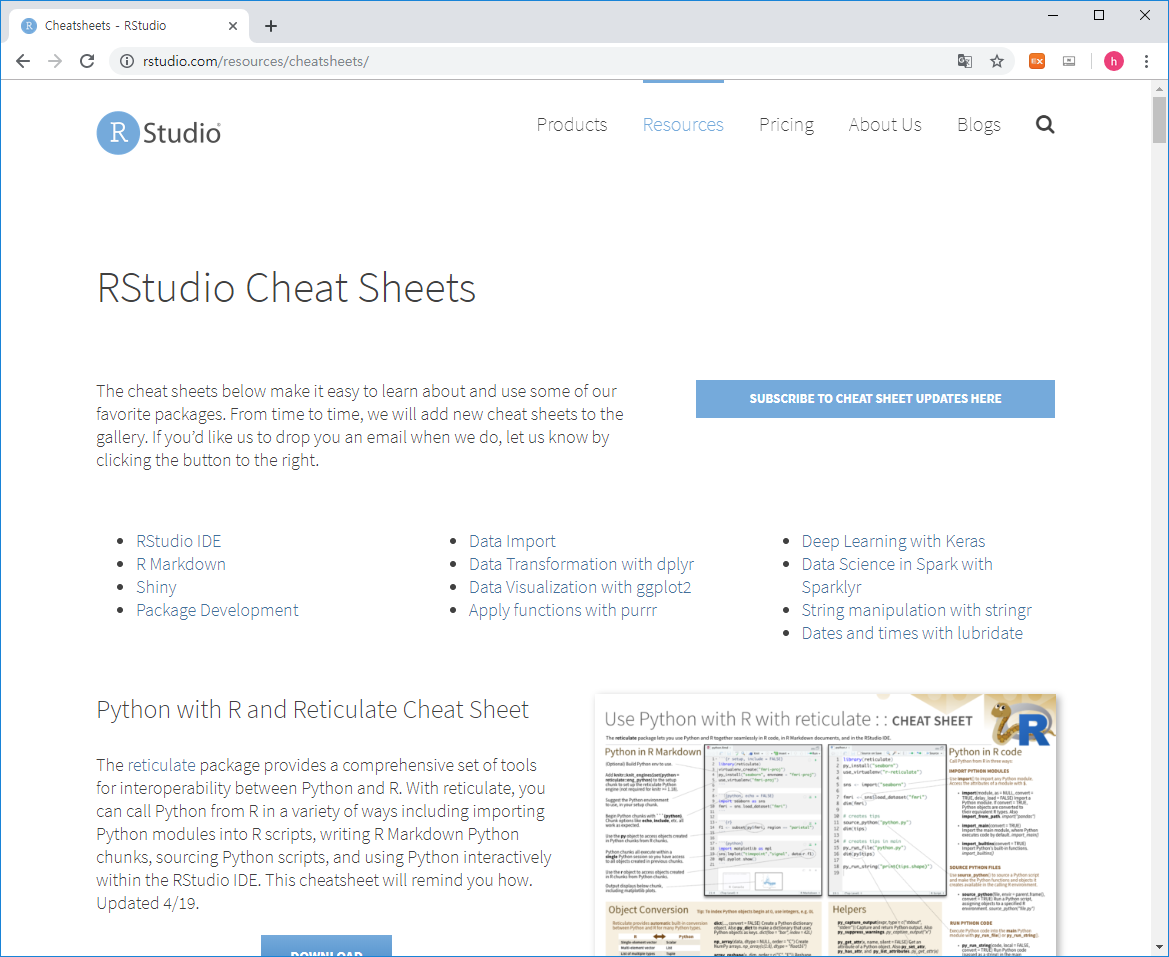
\includegraphics{images/01-16.PNG}
  \end{itemize}
\end{itemize}

\hypertarget{r-basics}{%
\chapter{R basics}\label{r-basics}}

\hypertarget{what-is-r-rstudio}{%
\section{What is R / Rstudio}\label{what-is-r-rstudio}}


\includegraphics{images/r.jpg}

\begin{itemize}
\tightlist
\item
  R is a programming language that runs computations (\url{https://www.r-project.org/})
\item
  RStudio is an integrated development environment (IDE) that provides an interface for the programming (\url{https://www.rstudio.com/})
\end{itemize}

\hypertarget{r-rstudio-installation}{%
\section{R / Rstudio installation}\label{r-rstudio-installation}}

\begin{itemize}
\item
  Install R first and then install RStudio second
\item
  R
  
\includegraphics{images/01-01.PNG}\\
  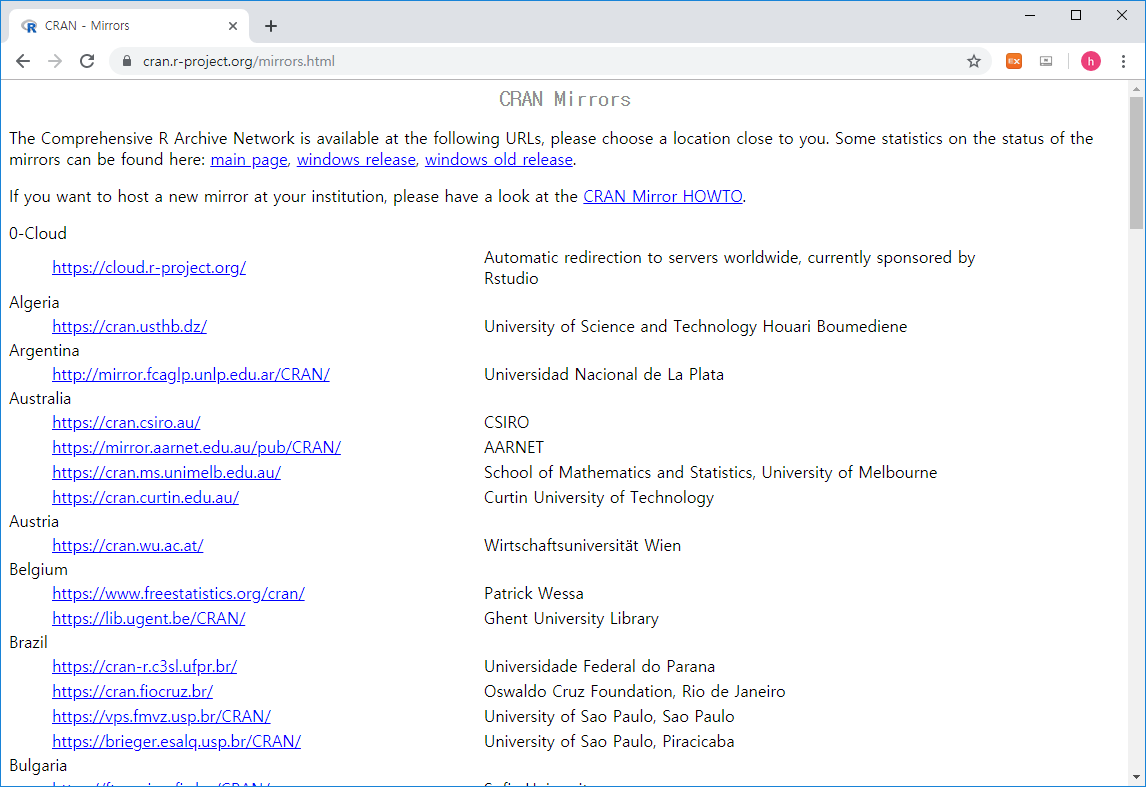
\includegraphics{images/01-02.PNG}\\
  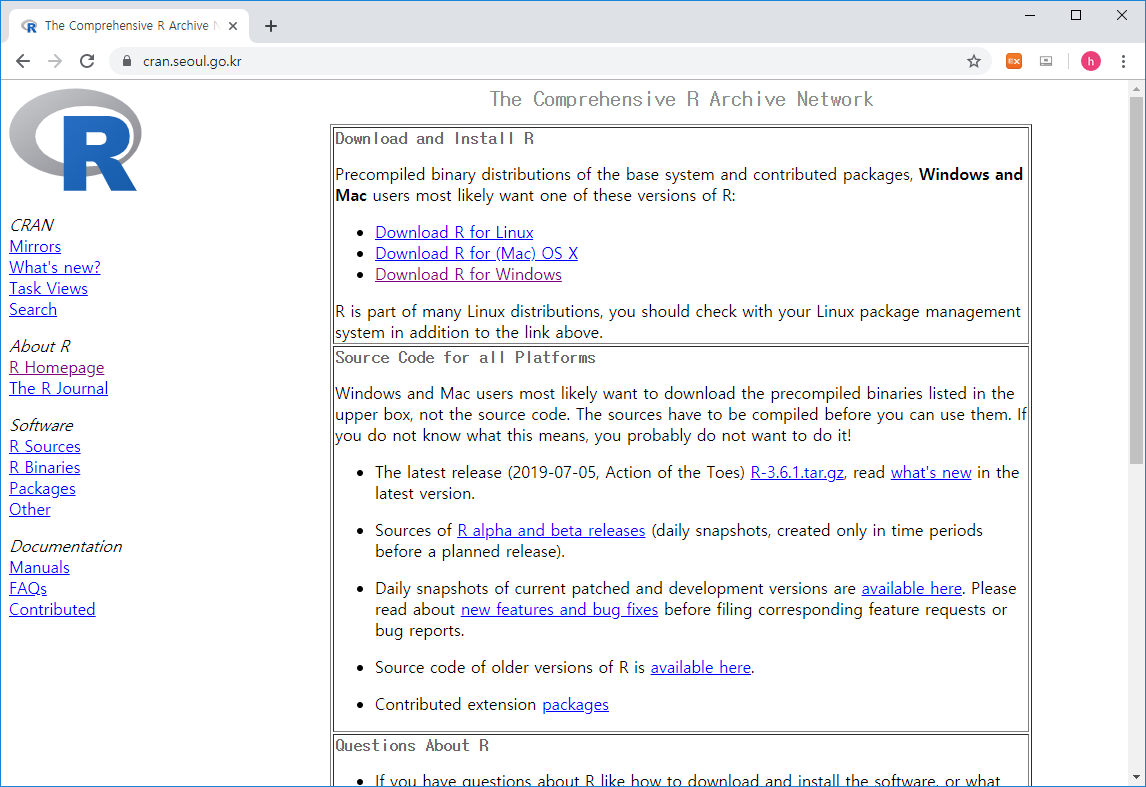
\includegraphics{images/01-03.PNG}\\
  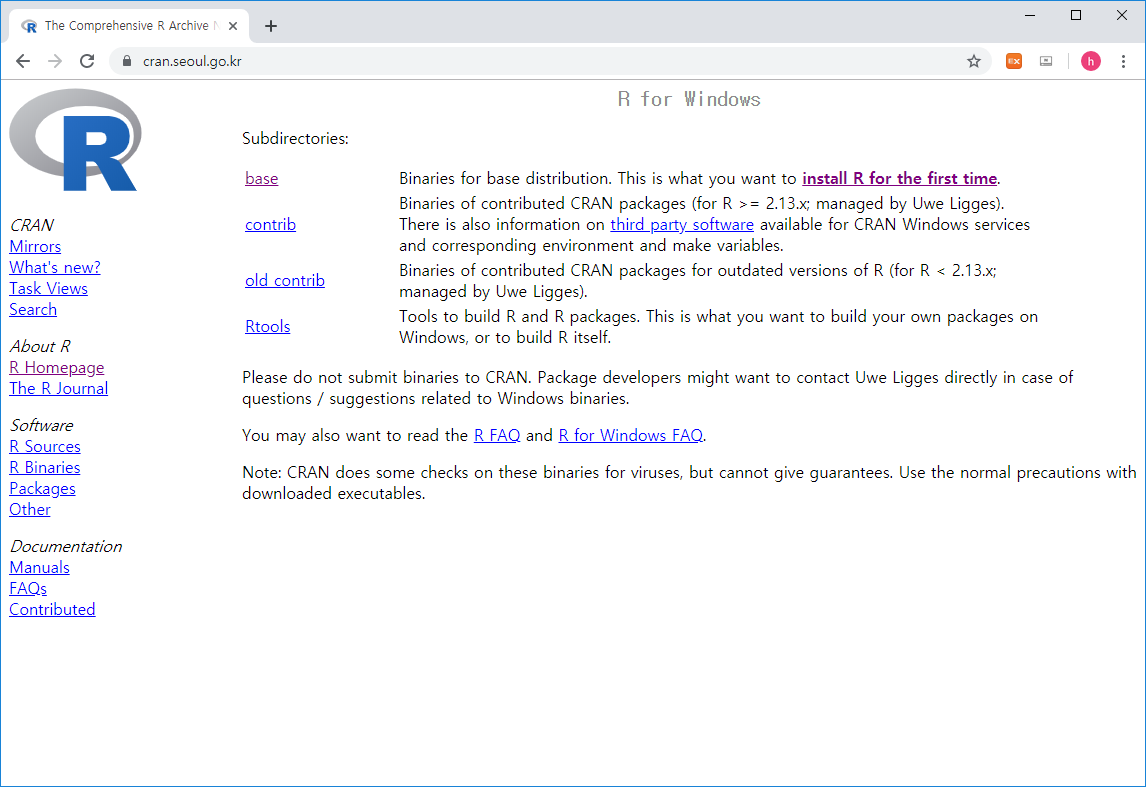
\includegraphics{images/01-04.PNG}\\
  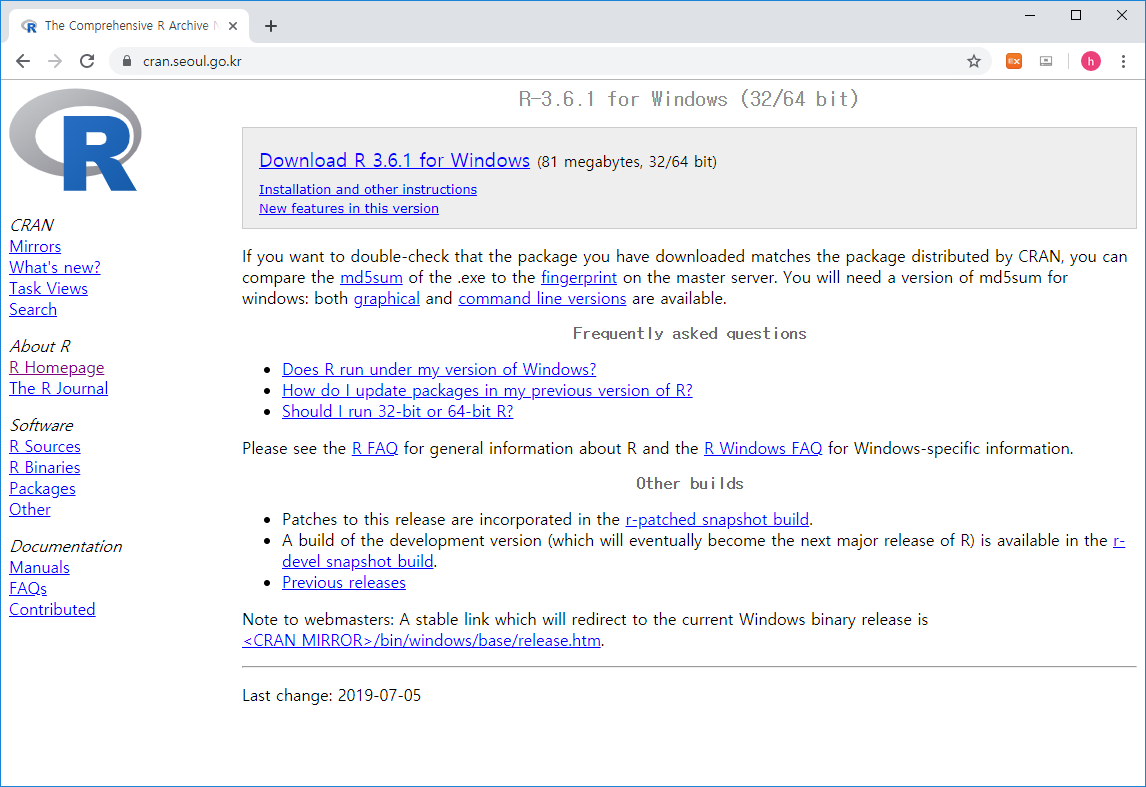
\includegraphics{images/01-05.PNG}
\item
  Rstudio
  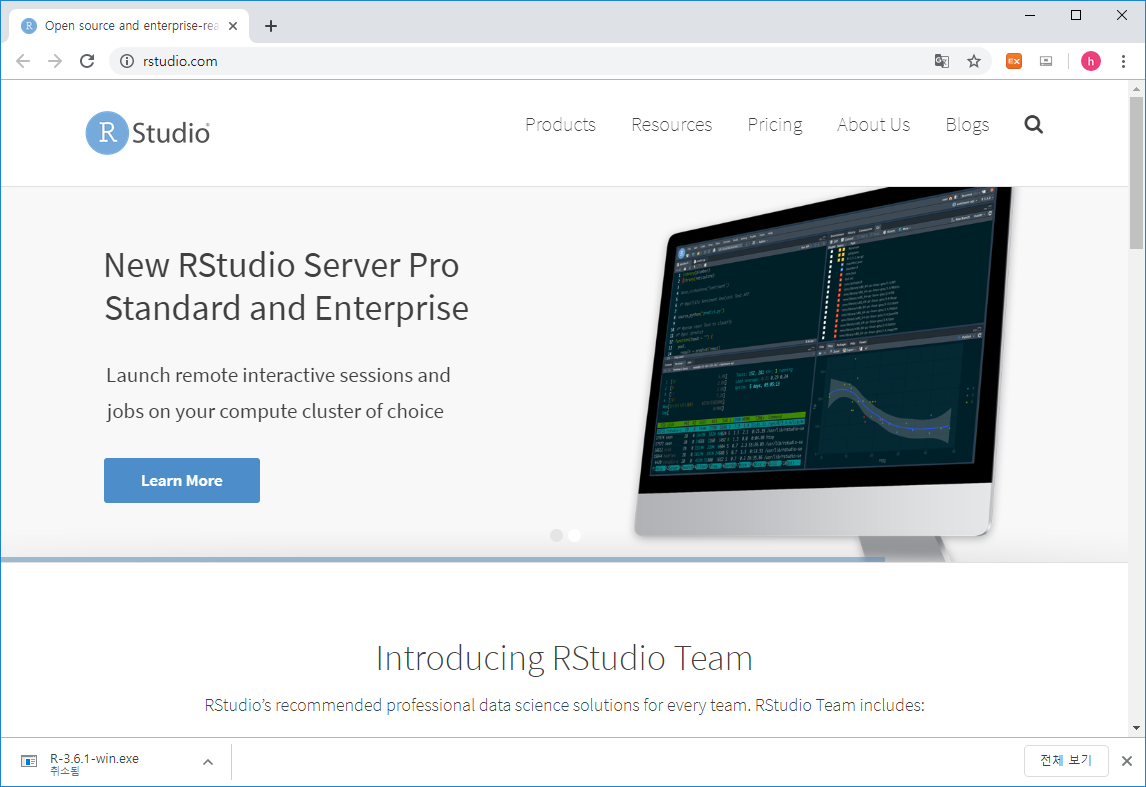
\includegraphics{images/01-06.PNG}\\
  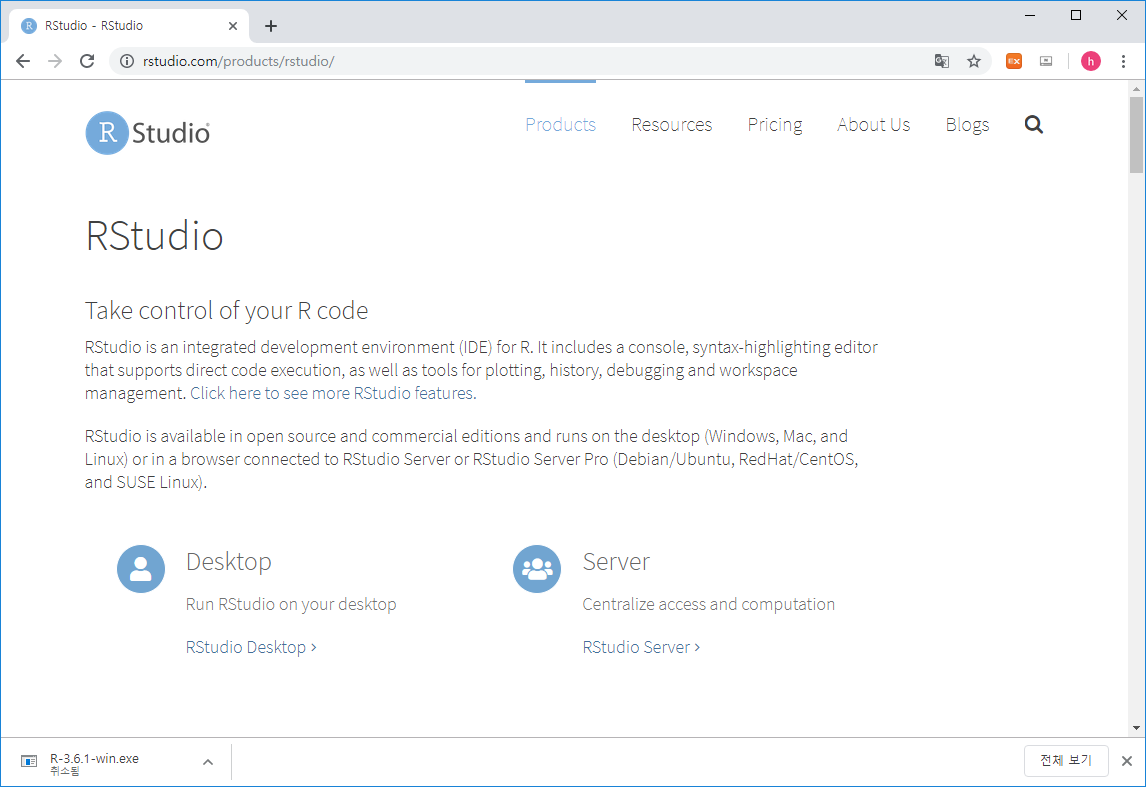
\includegraphics{images/01-07.PNG}\\
  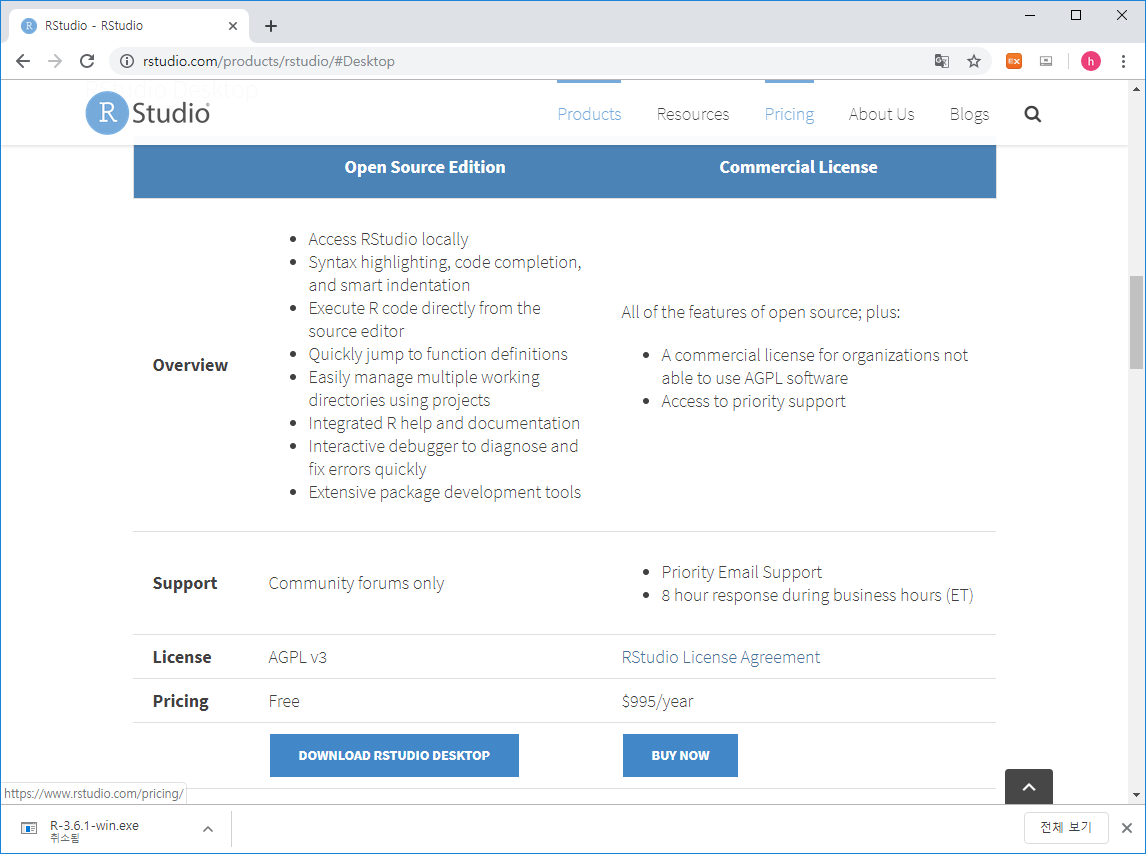
\includegraphics{images/01-08.PNG}\\
  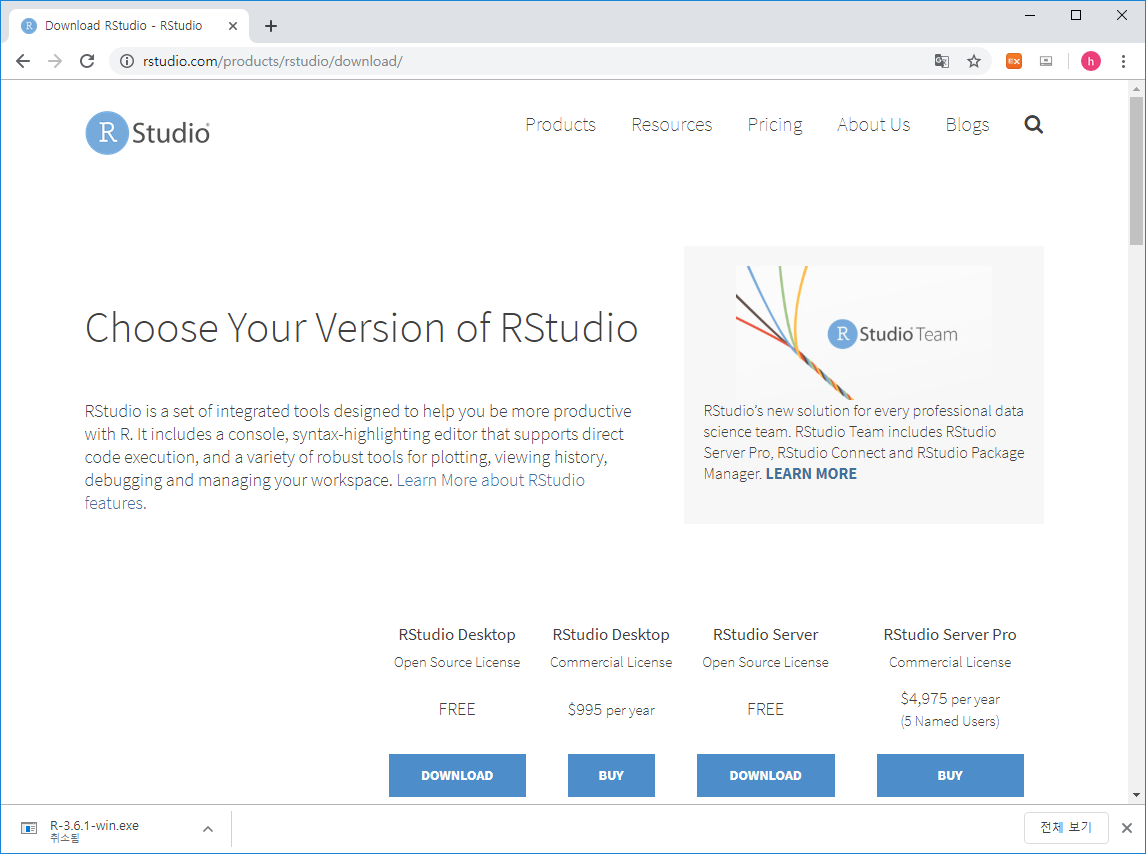
\includegraphics{images/01-09.PNG}\\
  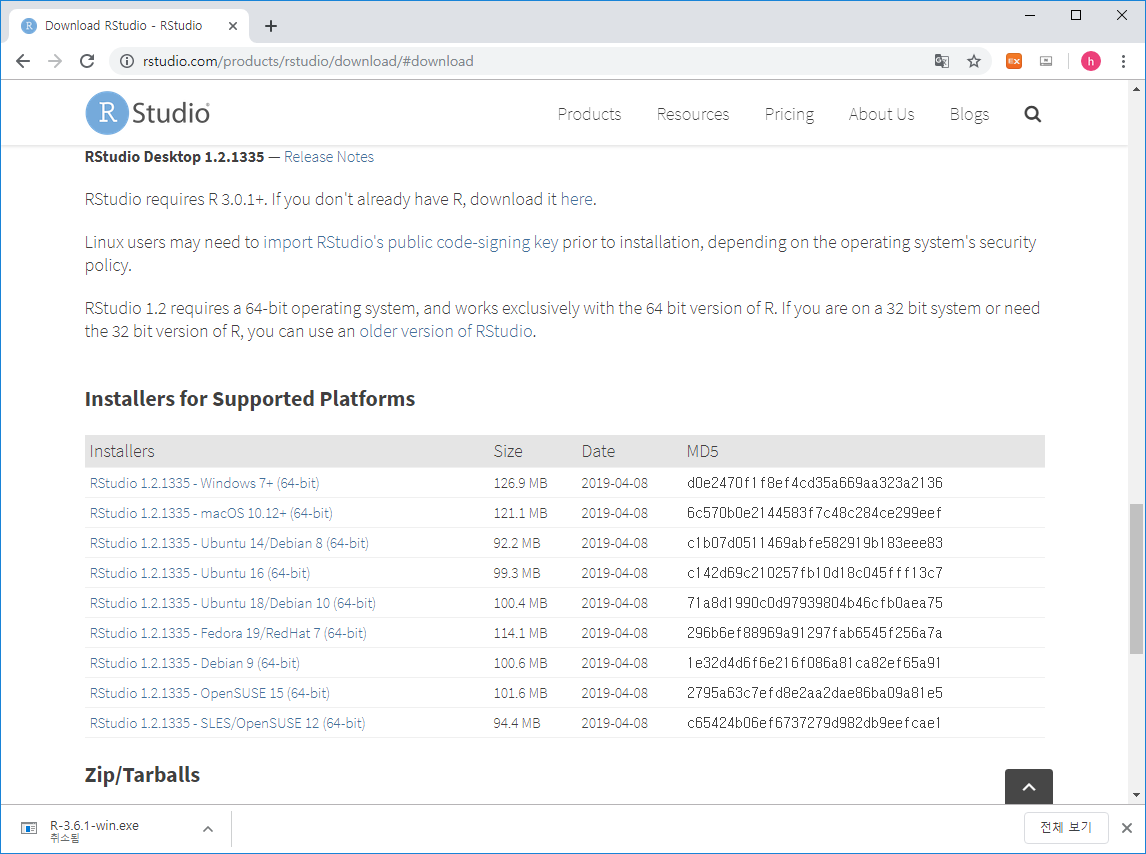
\includegraphics{images/01-10.PNG}
\end{itemize}

\hypertarget{rstudio-interface}{%
\section{Rstudio interface}\label{rstudio-interface}}

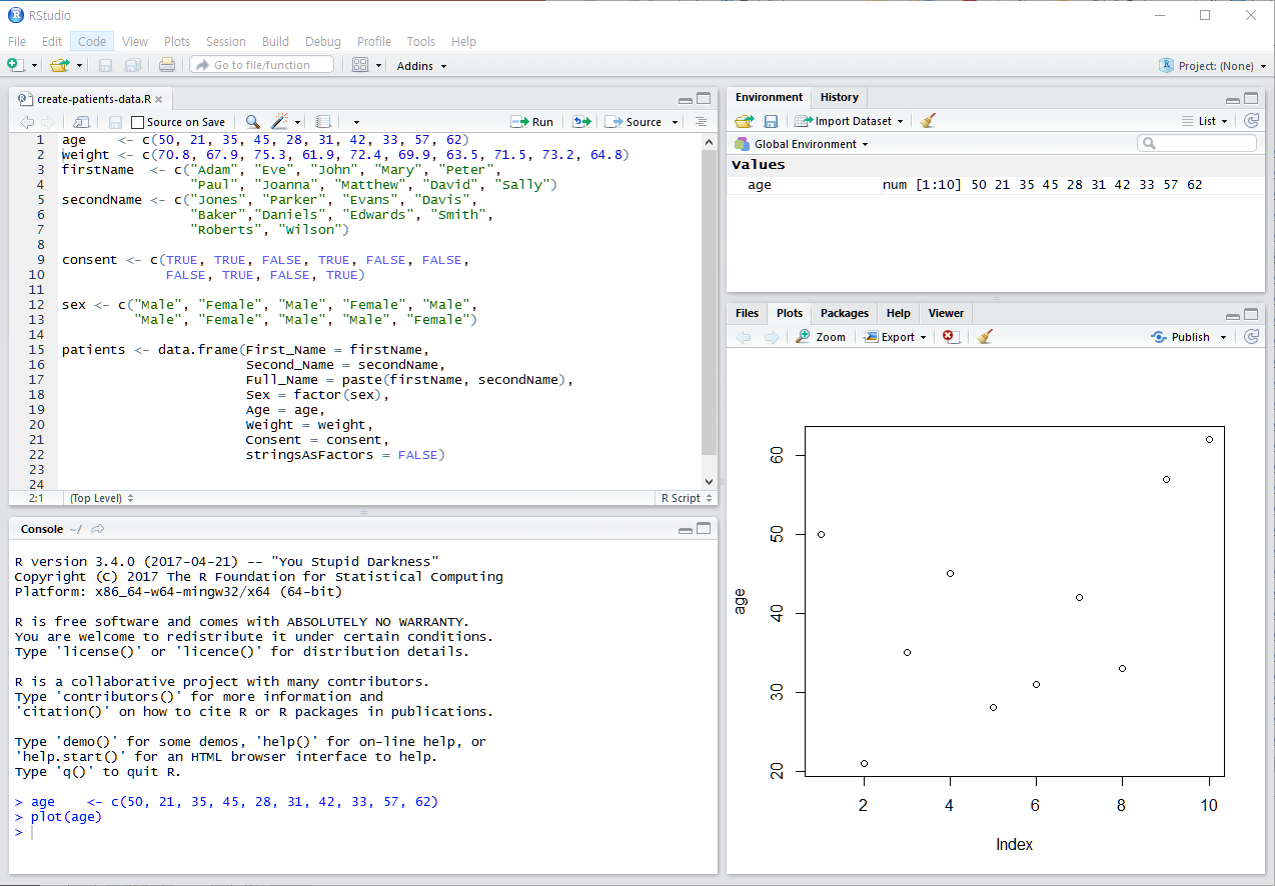
\includegraphics{images/01-11.PNG}

\hypertarget{keyboard-shortcuts}{%
\section{Keyboard shortcuts}\label{keyboard-shortcuts}}

\begin{itemize}
\item
  참고사이트

  \begin{itemize}
  \tightlist
  \item
    \url{https://support.rstudio.com/hc/en-us/articles/200711853-Keyboard-Shortcuts}
  \item
    Tools --\textgreater{} Keyboard shortcut Quick Reference (Alt + Shift + K)
  \end{itemize}
\item
  코드편집창 이동 (Ctrl+1) 콘솔창 이동(Ctrl+2)
\item
  한 줄 실행 (Ctrl+Enter)
\item
  주석처리 (Ctrl + Shift + C)

  \begin{itemize}
  \tightlist
  \item
    Starting with a hashmark (`\#'), everything to the end of the line is a comment
  \end{itemize}
\item
  실습

  \begin{itemize}
  \tightlist
  \item
    코드편집창에서 다음 입력
  \item
    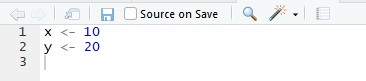
\includegraphics{images/01-14.PNG}\\
  \item
    단축키 Ctrl + enter로 코드 실행
  \item
    단축키 Ctrl + 2로 커서 콘솔창으로 이동
  \item
    x값 x+y값 확인
  \item
    단축키 Ctrl + 1로 코드편집창 이동
  \item
    단축키 Ctrl + Shift + C 사용
  \end{itemize}
\end{itemize}

\begin{Shaded}
\begin{Highlighting}[]
\CommentTok{# x <- 10}
\CommentTok{# y <- 20}
\end{Highlighting}
\end{Shaded}

\hypertarget{r-programming-basics-and-terminology}{%
\section{R programming basics and terminology}\label{r-programming-basics-and-terminology}}

\begin{itemize}
\tightlist
\item
  Console: 명령어 입력하는 창
\item
  Code: R 프로그래밍 변수/제어문 모음\\
\item
  Objects (개체, variable): 값이 (데이터) 저장되는 장소
\item
  Data types: Integers, doubles/numerics, logicals, and characters.
\item
  Object (Variable) types:

  \begin{itemize}
  \tightlist
  \item
    Vectors: 값들의 모임 combine function c() EX: c(6, 11, 13, 31, 90, 92)
  \item
    Factors: 범주형 데이터 저장 장소
  \item
    Data frames: 2D matrix 형태 데이터 자장 장소
  \end{itemize}
\item
  Conditionals (조건, 제어):

  \begin{itemize}
  \tightlist
  \item
    if: ==, \& (AND), \textbar{} (OR) Ex: (2 + 1 == 3) \& (2 + 1 == 4)
  \item
    for, while: 반복 수
  \end{itemize}
\item
  Functions (함수, commands): 특정 일 수행, 함수이름 - 입력값 (arguments) - 출력값 (output) 으로 구성
\end{itemize}

\hypertarget{set-working-directory}{%
\section{Set working directory}\label{set-working-directory}}

\begin{itemize}
\tightlist
\item
  시작 전 항상 작업 디렉토리 설정
\item
  예를 들어 c:~아래 새로운 디렉토리 rstat01 을 만들고 작업공간으로 설정
\end{itemize}

\begin{Shaded}
\begin{Highlighting}[]
\KeywordTok{getwd}\NormalTok{()}
\KeywordTok{dir}\NormalTok{()}
\KeywordTok{setwd}\NormalTok{(}\StringTok{"C:}\CharTok{\textbackslash{}\textbackslash{}}\StringTok{rstat01"}\NormalTok{)}
\KeywordTok{getwd}\NormalTok{()}
\KeywordTok{dir}\NormalTok{()}
\end{Highlighting}
\end{Shaded}

\begin{itemize}
\tightlist
\item
  또는 아래와 같이 RStudio 메뉴 에서 설정
  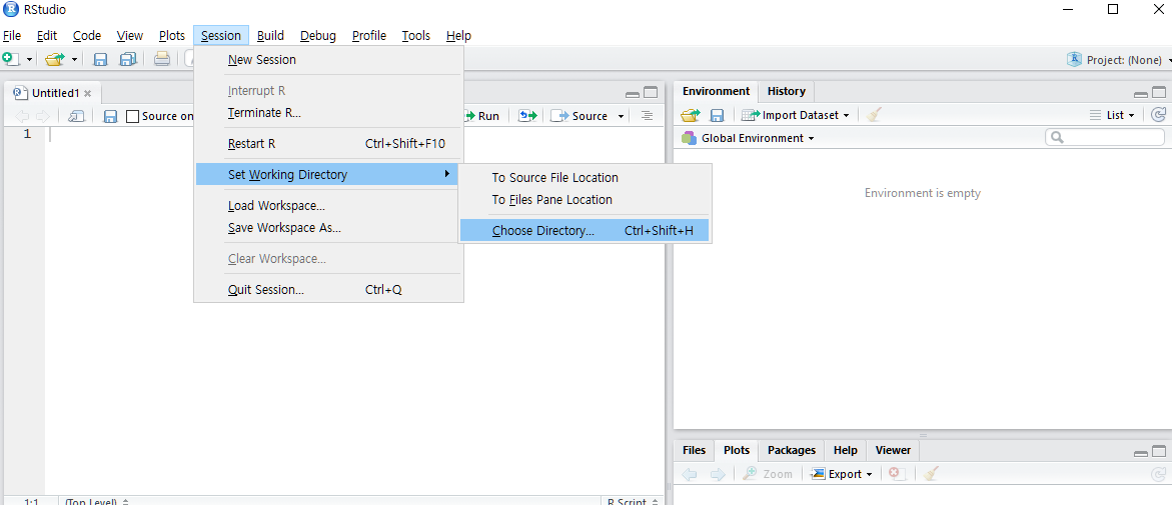
\includegraphics{images/01-12.PNG}
\end{itemize}

\hypertarget{r-coding-practice}{%
\section{R coding practice}\label{r-coding-practice}}

\begin{itemize}
\tightlist
\item
  콘솔 계산기
\end{itemize}

\begin{Shaded}
\begin{Highlighting}[]
\DecValTok{2} \OperatorTok{+}\StringTok{ }\DecValTok{2}
\NormalTok{((}\DecValTok{2}\NormalTok{ – }\DecValTok{1}\NormalTok{)}\OperatorTok{^}\DecValTok{2} \OperatorTok{+}\StringTok{ }\NormalTok{(}\DecValTok{1}\NormalTok{ – }\DecValTok{3}\NormalTok{)}\OperatorTok{^}\DecValTok{2}\NormalTok{ )}\OperatorTok{^}\NormalTok{(}\DecValTok{1}\OperatorTok{/}\DecValTok{2}\NormalTok{)}
\DecValTok{2} \OperatorTok{+}\StringTok{ }\DecValTok{2}\NormalTok{; }\DecValTok{2} \OperatorTok{-}\StringTok{ }\DecValTok{2}
\end{Highlighting}
\end{Shaded}

\begin{itemize}
\tightlist
\item
  이전 명령: 콘솔에서 위 아래 화살표
\end{itemize}

\hypertarget{variables-and-values}{%
\section{Variables and values}\label{variables-and-values}}

\begin{itemize}
\tightlist
\item
  R is a programming language
\item
  Assignment operator ( \texttt{\textless{}-} OR \texttt{=} )

  \begin{itemize}
  \tightlist
  \item
    Valid object name \texttt{\textless{}-} value
  \item
    단축키: \texttt{Alt\ +\ -} (the minus sign)
  \end{itemize}
\item
  내장 변수 Built-in variables
\end{itemize}

\begin{Shaded}
\begin{Highlighting}[]
\NormalTok{x <-}\StringTok{ }\DecValTok{2}
\NormalTok{y <-}\StringTok{ }\NormalTok{x}\OperatorTok{^}\DecValTok{2}\NormalTok{ – }\DecValTok{2}\OperatorTok{*}\NormalTok{x }\OperatorTok{+}\StringTok{ }\DecValTok{1}
\NormalTok{y}
\NormalTok{x <-}\StringTok{ "two"}  
\NormalTok{some_data <-}\StringTok{ }\FloatTok{9.8}
\NormalTok{pi}
\end{Highlighting}
\end{Shaded}

\begin{itemize}
\tightlist
\item
  변수이름 작명법

  \begin{itemize}
  \tightlist
  \item
    Characters (letters), numbers, ``\_'', ``.''
  \item
    A and a are different symbols
  \item
    Names are effectively unlimited in length
  \end{itemize}
\end{itemize}

\begin{Shaded}
\begin{Highlighting}[]
\NormalTok{i_use_snake_case <-}\StringTok{ }\DecValTok{1}
\NormalTok{otherPeopleUseCamelCase <-}\StringTok{ }\DecValTok{2}
\NormalTok{some.people.use.periods <-}\StringTok{ }\DecValTok{3}
\NormalTok{And_aFew.People_RENOUNCEconvention <-}\StringTok{ }\DecValTok{4}
\end{Highlighting}
\end{Shaded}

\begin{itemize}
\tightlist
\item
  자동 완성 기능 (Tab completion) in RStudio
\end{itemize}

\hypertarget{variable-type-of-storage-mode}{%
\section{Variable type of (storage) mode}\label{variable-type-of-storage-mode}}

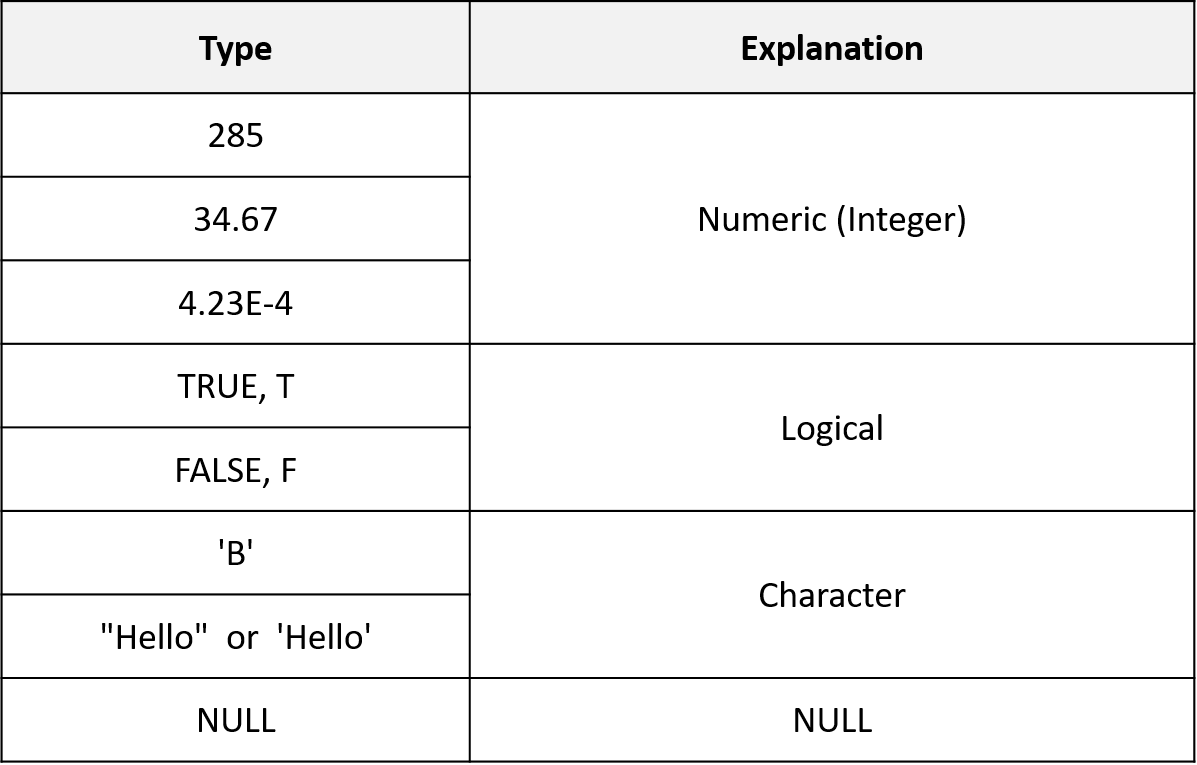
\includegraphics{images/01-13.PNG}

\hypertarget{variable---vectors}{%
\section{Variable - Vectors}\label{variable---vectors}}

\begin{itemize}
\tightlist
\item
  Combine function \texttt{c()}: Concatenating elements end to end
\end{itemize}

\begin{Shaded}
\begin{Highlighting}[]
\NormalTok{x <-}\StringTok{ }\KeywordTok{c}\NormalTok{(}\FloatTok{10.4}\NormalTok{, }\FloatTok{5.6}\NormalTok{, }\FloatTok{3.1}\NormalTok{, }\FloatTok{6.4}\NormalTok{, }\FloatTok{21.7}\NormalTok{) }
\NormalTok{y <-}\StringTok{ }\KeywordTok{c}\NormalTok{(}\StringTok{"X1"}\NormalTok{, }\StringTok{"Y2"}\NormalTok{,  }\StringTok{"X3"}\NormalTok{,  }\StringTok{"Y4"}\NormalTok{)}
\end{Highlighting}
\end{Shaded}

\begin{itemize}
\tightlist
\item
  인덱싱: Subsets of the elements of a vector
\end{itemize}

\begin{Shaded}
\begin{Highlighting}[]
\NormalTok{x[}\DecValTok{1}\NormalTok{]}
\NormalTok{x[}\DecValTok{1}\OperatorTok{:}\DecValTok{3}\NormalTok{]}
\NormalTok{x[}\KeywordTok{c}\NormalTok{(}\DecValTok{1}\NormalTok{,}\DecValTok{2}\NormalTok{,}\DecValTok{4}\NormalTok{)]}
\NormalTok{y[}\DecValTok{3}\NormalTok{]}
\end{Highlighting}
\end{Shaded}

\hypertarget{functions}{%
\section{Functions}\label{functions}}

\begin{itemize}
\tightlist
\item
  Function define
\end{itemize}

\begin{Shaded}
\begin{Highlighting}[]
\NormalTok{my_sine <-}\StringTok{ }\ControlFlowTok{function}\NormalTok{(x)\{}
\NormalTok{    y <-}\StringTok{ }\KeywordTok{sin}\NormalTok{(x)}
    \KeywordTok{return}\NormalTok{(y)}
\NormalTok{\}}
\end{Highlighting}
\end{Shaded}

\begin{itemize}
\tightlist
\item
  Usage
\end{itemize}

\begin{Shaded}
\begin{Highlighting}[]
\KeywordTok{my_sine}\NormalTok{(pi)}
\end{Highlighting}
\end{Shaded}

\begin{itemize}
\tightlist
\item
  Terminology

  \begin{itemize}
  \tightlist
  \item
    function name: \texttt{my\_sine}
  \item
    parameter: \texttt{x}
  \item
    argument: \texttt{pi}
  \item
    return value: \texttt{y}
  \end{itemize}
\item
  Built-in functions

  \begin{itemize}
  \tightlist
  \item
    Arguments separated by commas
  \item
    Tab completion
  \end{itemize}
\end{itemize}

\begin{Shaded}
\begin{Highlighting}[]
\NormalTok{x <-}\StringTok{ }\NormalTok{pi}
\KeywordTok{sin}\NormalTok{(x)}
\KeywordTok{sqrt}\NormalTok{(x)}
\KeywordTok{log}\NormalTok{(x)}
\KeywordTok{log}\NormalTok{(x, }\DecValTok{10}\NormalTok{)}
\NormalTok{x <-}\StringTok{ }\KeywordTok{c}\NormalTok{(}\DecValTok{10}\NormalTok{, }\DecValTok{20}\NormalTok{, }\DecValTok{30}\NormalTok{)}
\NormalTok{x }\OperatorTok{+}\StringTok{ }\NormalTok{x}
\KeywordTok{mean}\NormalTok{(x)}
\KeywordTok{sum}\NormalTok{(x)}\OperatorTok{/}\KeywordTok{length}\NormalTok{(x)}
\end{Highlighting}
\end{Shaded}

\hypertarget{vectorized-functions}{%
\section{Vectorized functions}\label{vectorized-functions}}

\begin{Shaded}
\begin{Highlighting}[]
\NormalTok{x <-}\StringTok{ }\KeywordTok{c}\NormalTok{(}\DecValTok{10}\NormalTok{, }\DecValTok{20}\NormalTok{, }\DecValTok{30}\NormalTok{)}
\NormalTok{x }\OperatorTok{+}\StringTok{ }\NormalTok{x}
\KeywordTok{sqrt}\NormalTok{(x)}
\KeywordTok{sin}\NormalTok{(x)}
\KeywordTok{log}\NormalTok{(x)}
\NormalTok{x}\OperatorTok{-}\KeywordTok{mean}\NormalTok{(x)}
\end{Highlighting}
\end{Shaded}

\hypertarget{help}{%
\section{Help}\label{help}}

\begin{itemize}
\tightlist
\item
  R의 장점 중 하나 (예제 포함)
\end{itemize}

\begin{Shaded}
\begin{Highlighting}[]
\NormalTok{?}
\NormalTok{?mean}
\KeywordTok{help}\NormalTok{(}\StringTok{"mean"}\NormalTok{)}
\KeywordTok{example}\NormalTok{(}\StringTok{"mean"}\NormalTok{)}
\KeywordTok{help.search}\NormalTok{(}\StringTok{"mean"}\NormalTok{)}
\KeywordTok{help}\NormalTok{(}\DataTypeTok{package=}\StringTok{"MASS"}\NormalTok{)}
\end{Highlighting}
\end{Shaded}

\hypertarget{rstudio-workspace}{%
\section{RStudio workspace}\label{rstudio-workspace}}

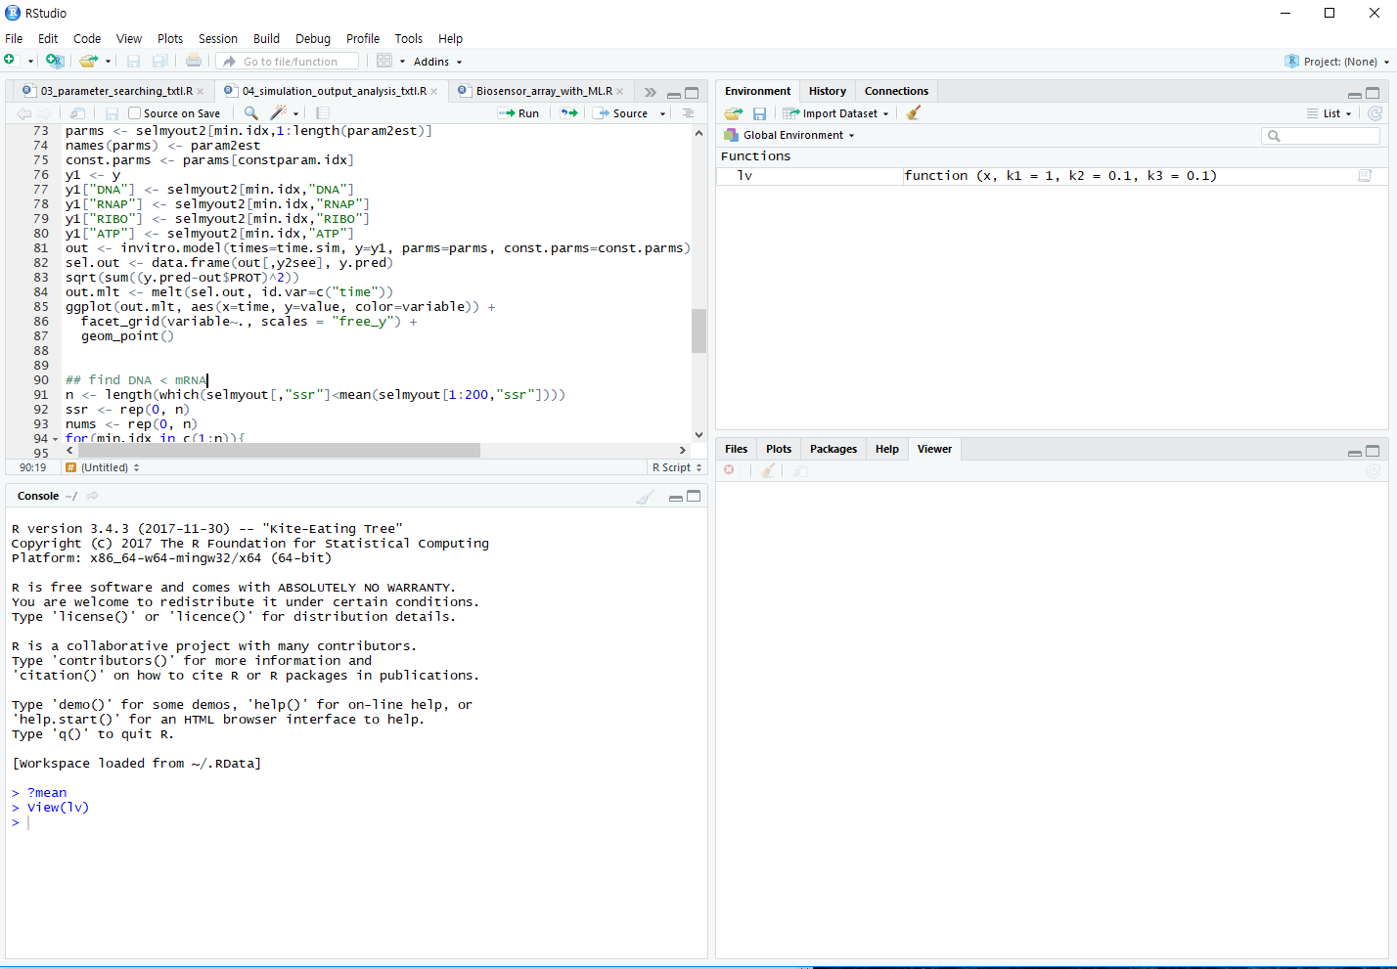
\includegraphics{images/01-17.PNG}
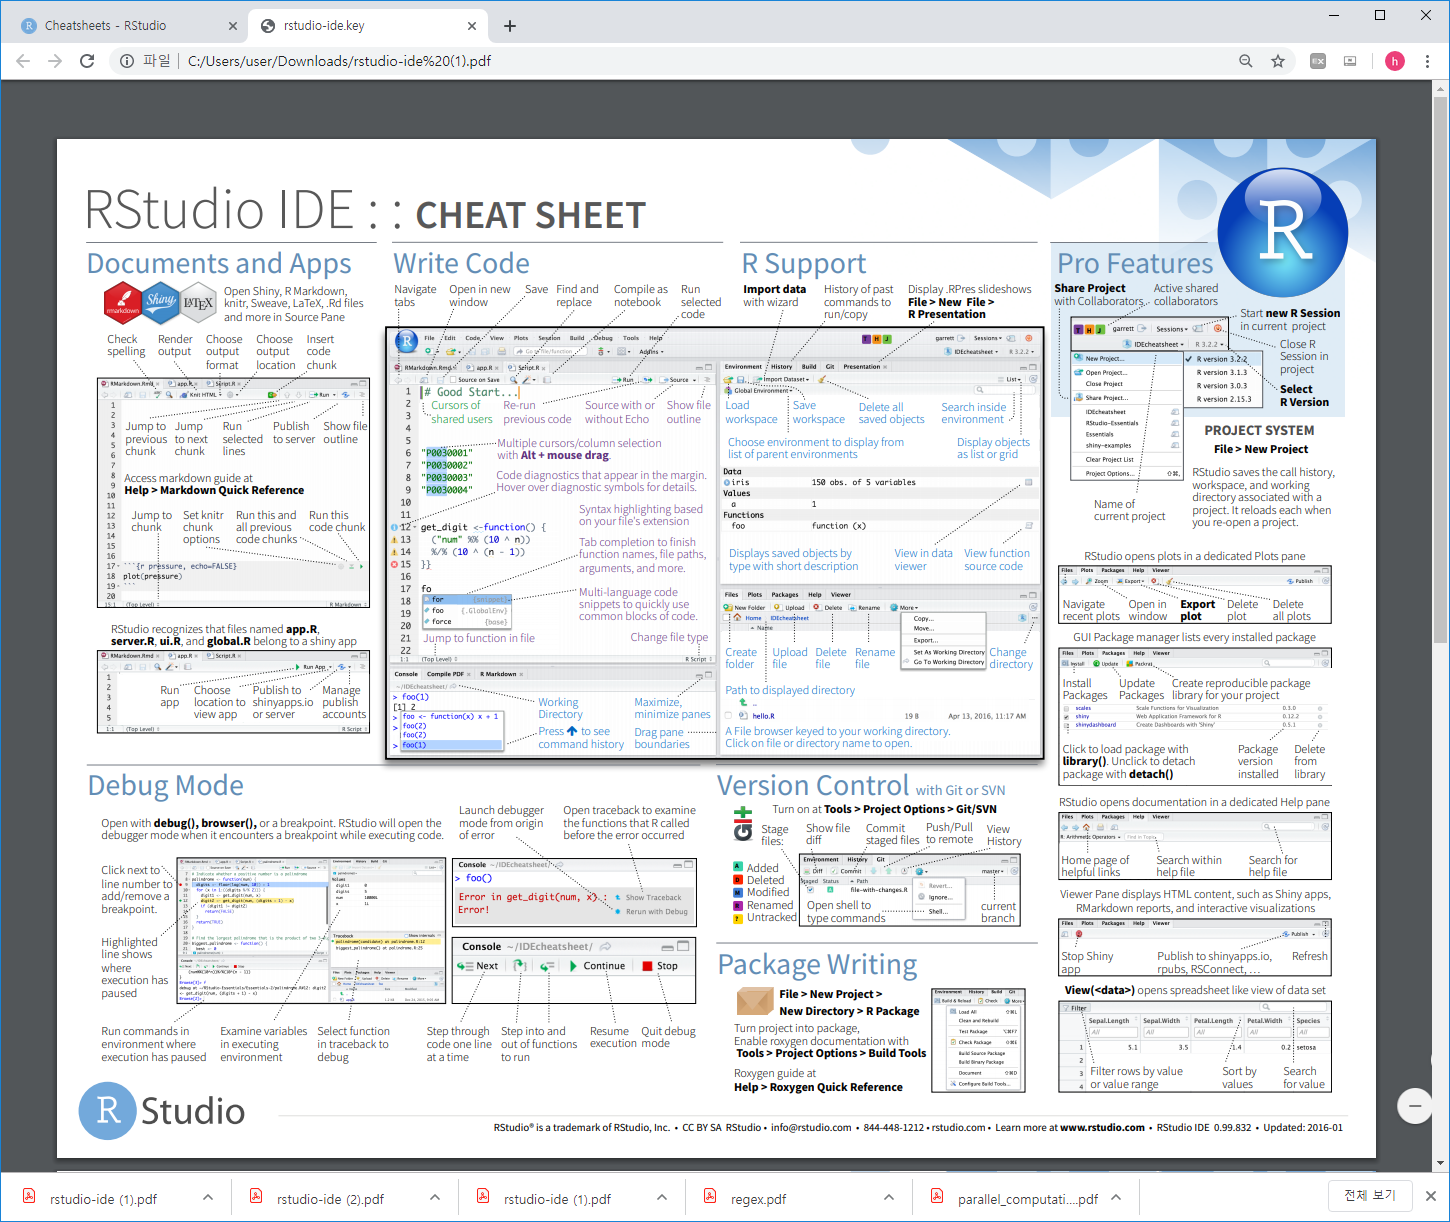
\includegraphics{images/rstudio-ide-1.png}
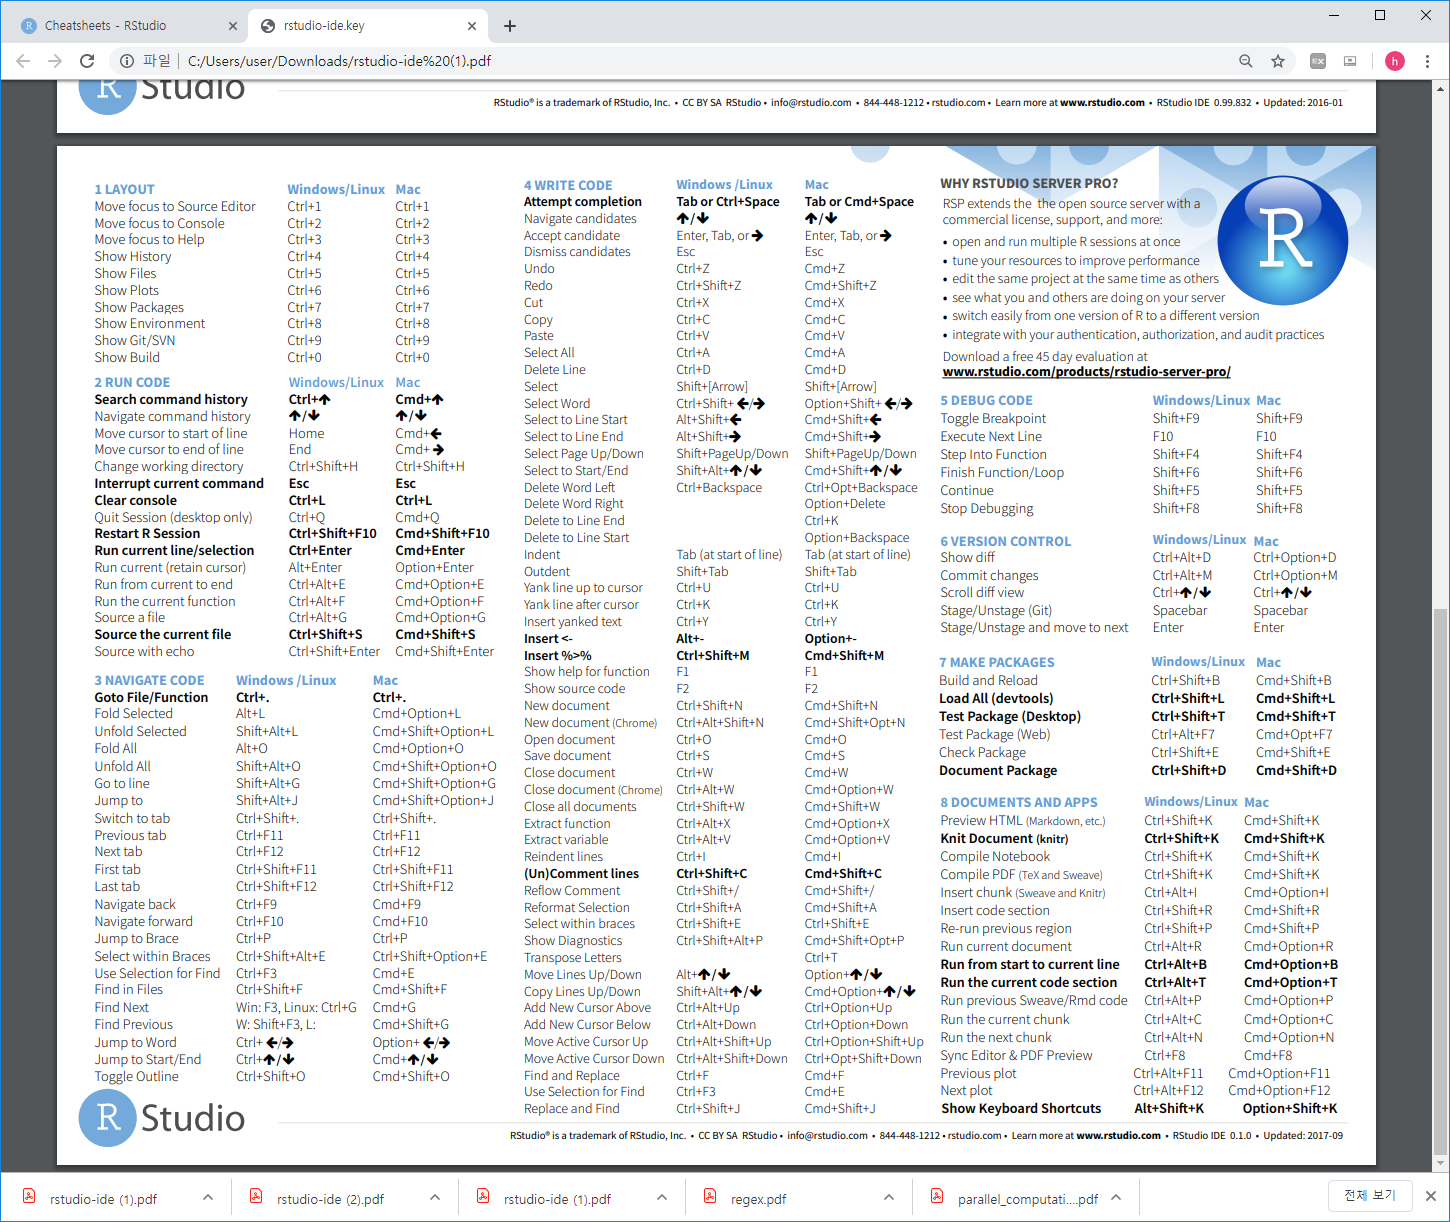
\includegraphics{images/rstudio-ide-2.png}

\hypertarget{r-packages}{%
\section{R packages}\label{r-packages}}

\begin{itemize}
\tightlist
\item
  R comes ready loaded with various libraries of functions called packages
\item
  ex) sum() is in the ``base'' package and sd() in the ``stats'' package
\item
  The packages can be found in numerous server locations on the web called repositories
\item
  The Comprehensive R Archive Network (CRAN) \url{http://cran.r-project.org/web/views/}
\item
  Bioconductor specialised in genomics \url{http://www.bioconductor.org/packages/release/bioc/}
\end{itemize}

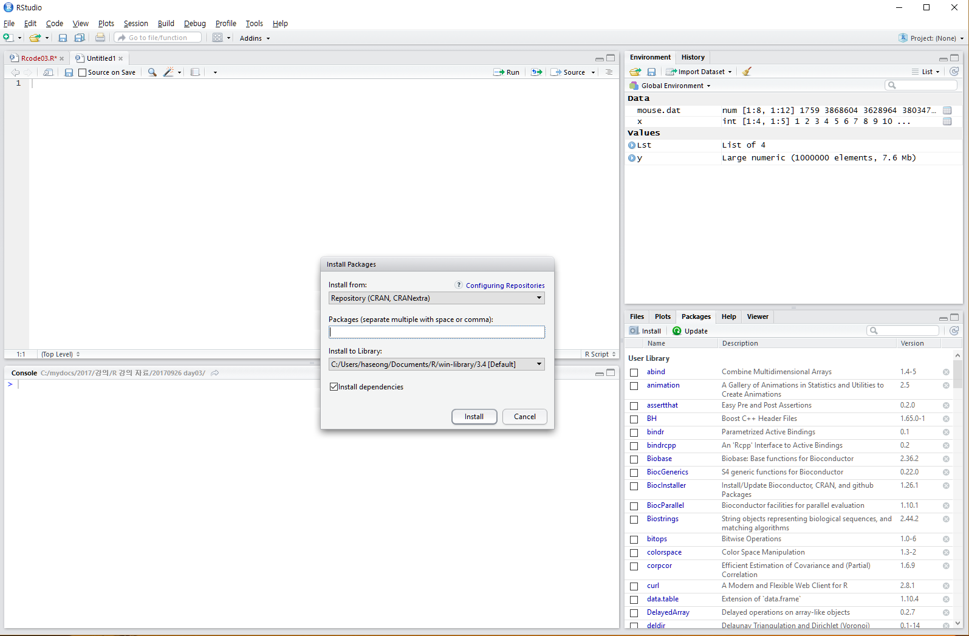
\includegraphics{images/01-18.png}

\begin{itemize}
\tightlist
\item
  UsingR package installation
\end{itemize}

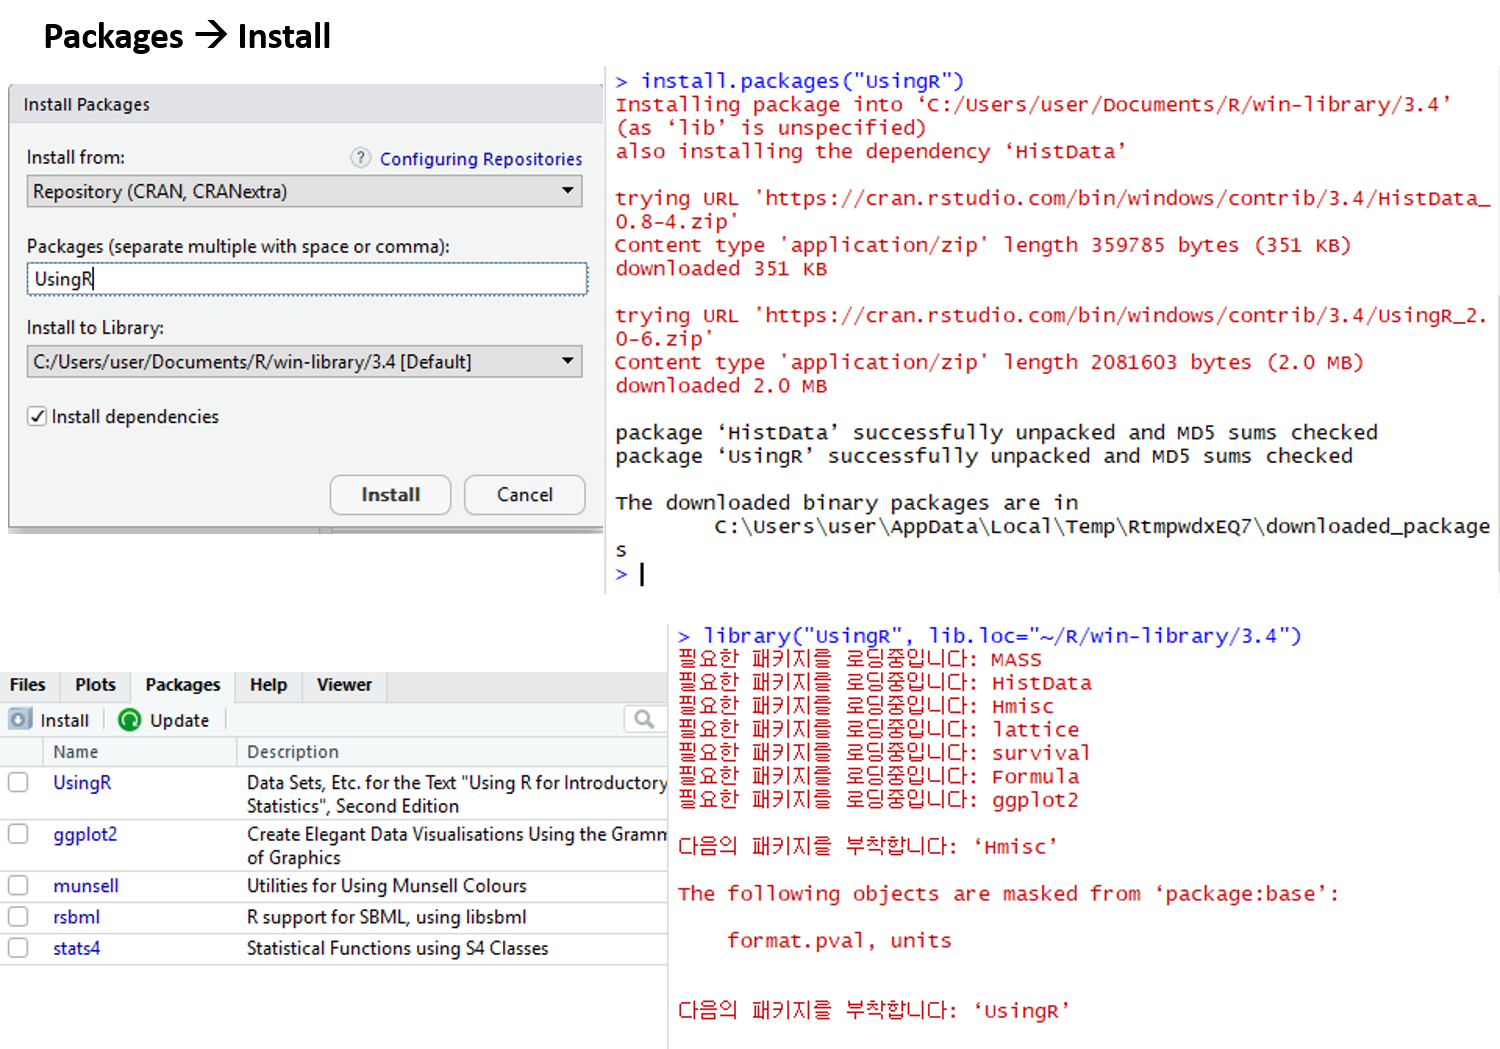
\includegraphics{images/01-19.png}

\begin{itemize}
\tightlist
\item
  UsingR package loading
\end{itemize}

\begin{Shaded}
\begin{Highlighting}[]
\KeywordTok{library}\NormalTok{(UsingR)}
\end{Highlighting}
\end{Shaded}

\begin{itemize}
\tightlist
\item
  R 설치 디렉토리
\item
  R 패키지 설치 디렉토리
\end{itemize}

\begin{Shaded}
\begin{Highlighting}[]
\KeywordTok{.libPaths}\NormalTok{()}
\KeywordTok{path.package}\NormalTok{()}
\end{Highlighting}
\end{Shaded}

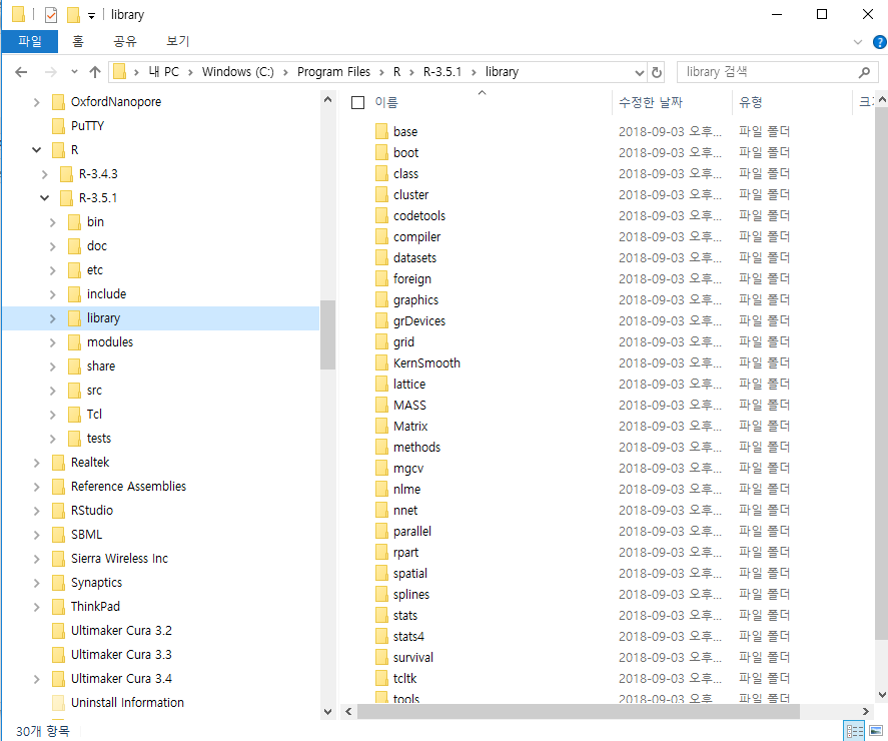
\includegraphics{images/01-20.png}

\hypertarget{data-sets}{%
\section{Data sets}\label{data-sets}}

\begin{itemize}
\tightlist
\item
  Packages include accompanying data sets
\item
  R has a datasets package that is loaded automatically
\item
  The data function produces a copy of dataset in user's workspace
\end{itemize}

\begin{Shaded}
\begin{Highlighting}[]
\KeywordTok{head}\NormalTok{(rivers)}
\KeywordTok{length}\NormalTok{(rivers)}
\KeywordTok{class}\NormalTok{(rivers)}
\KeywordTok{data}\NormalTok{(rivers)}
\KeywordTok{data}\NormalTok{(}\DataTypeTok{package=}\StringTok{"UsingR"}\NormalTok{)}
\KeywordTok{library}\NormalTok{(HistData)}
\KeywordTok{head}\NormalTok{(Cavendish)}
\KeywordTok{str}\NormalTok{(Cavendish)}
\KeywordTok{head}\NormalTok{(Cavendish}\OperatorTok{$}\NormalTok{density2)}
\end{Highlighting}
\end{Shaded}

\hypertarget{cheatsheet}{%
\section{Cheatsheet}\label{cheatsheet}}

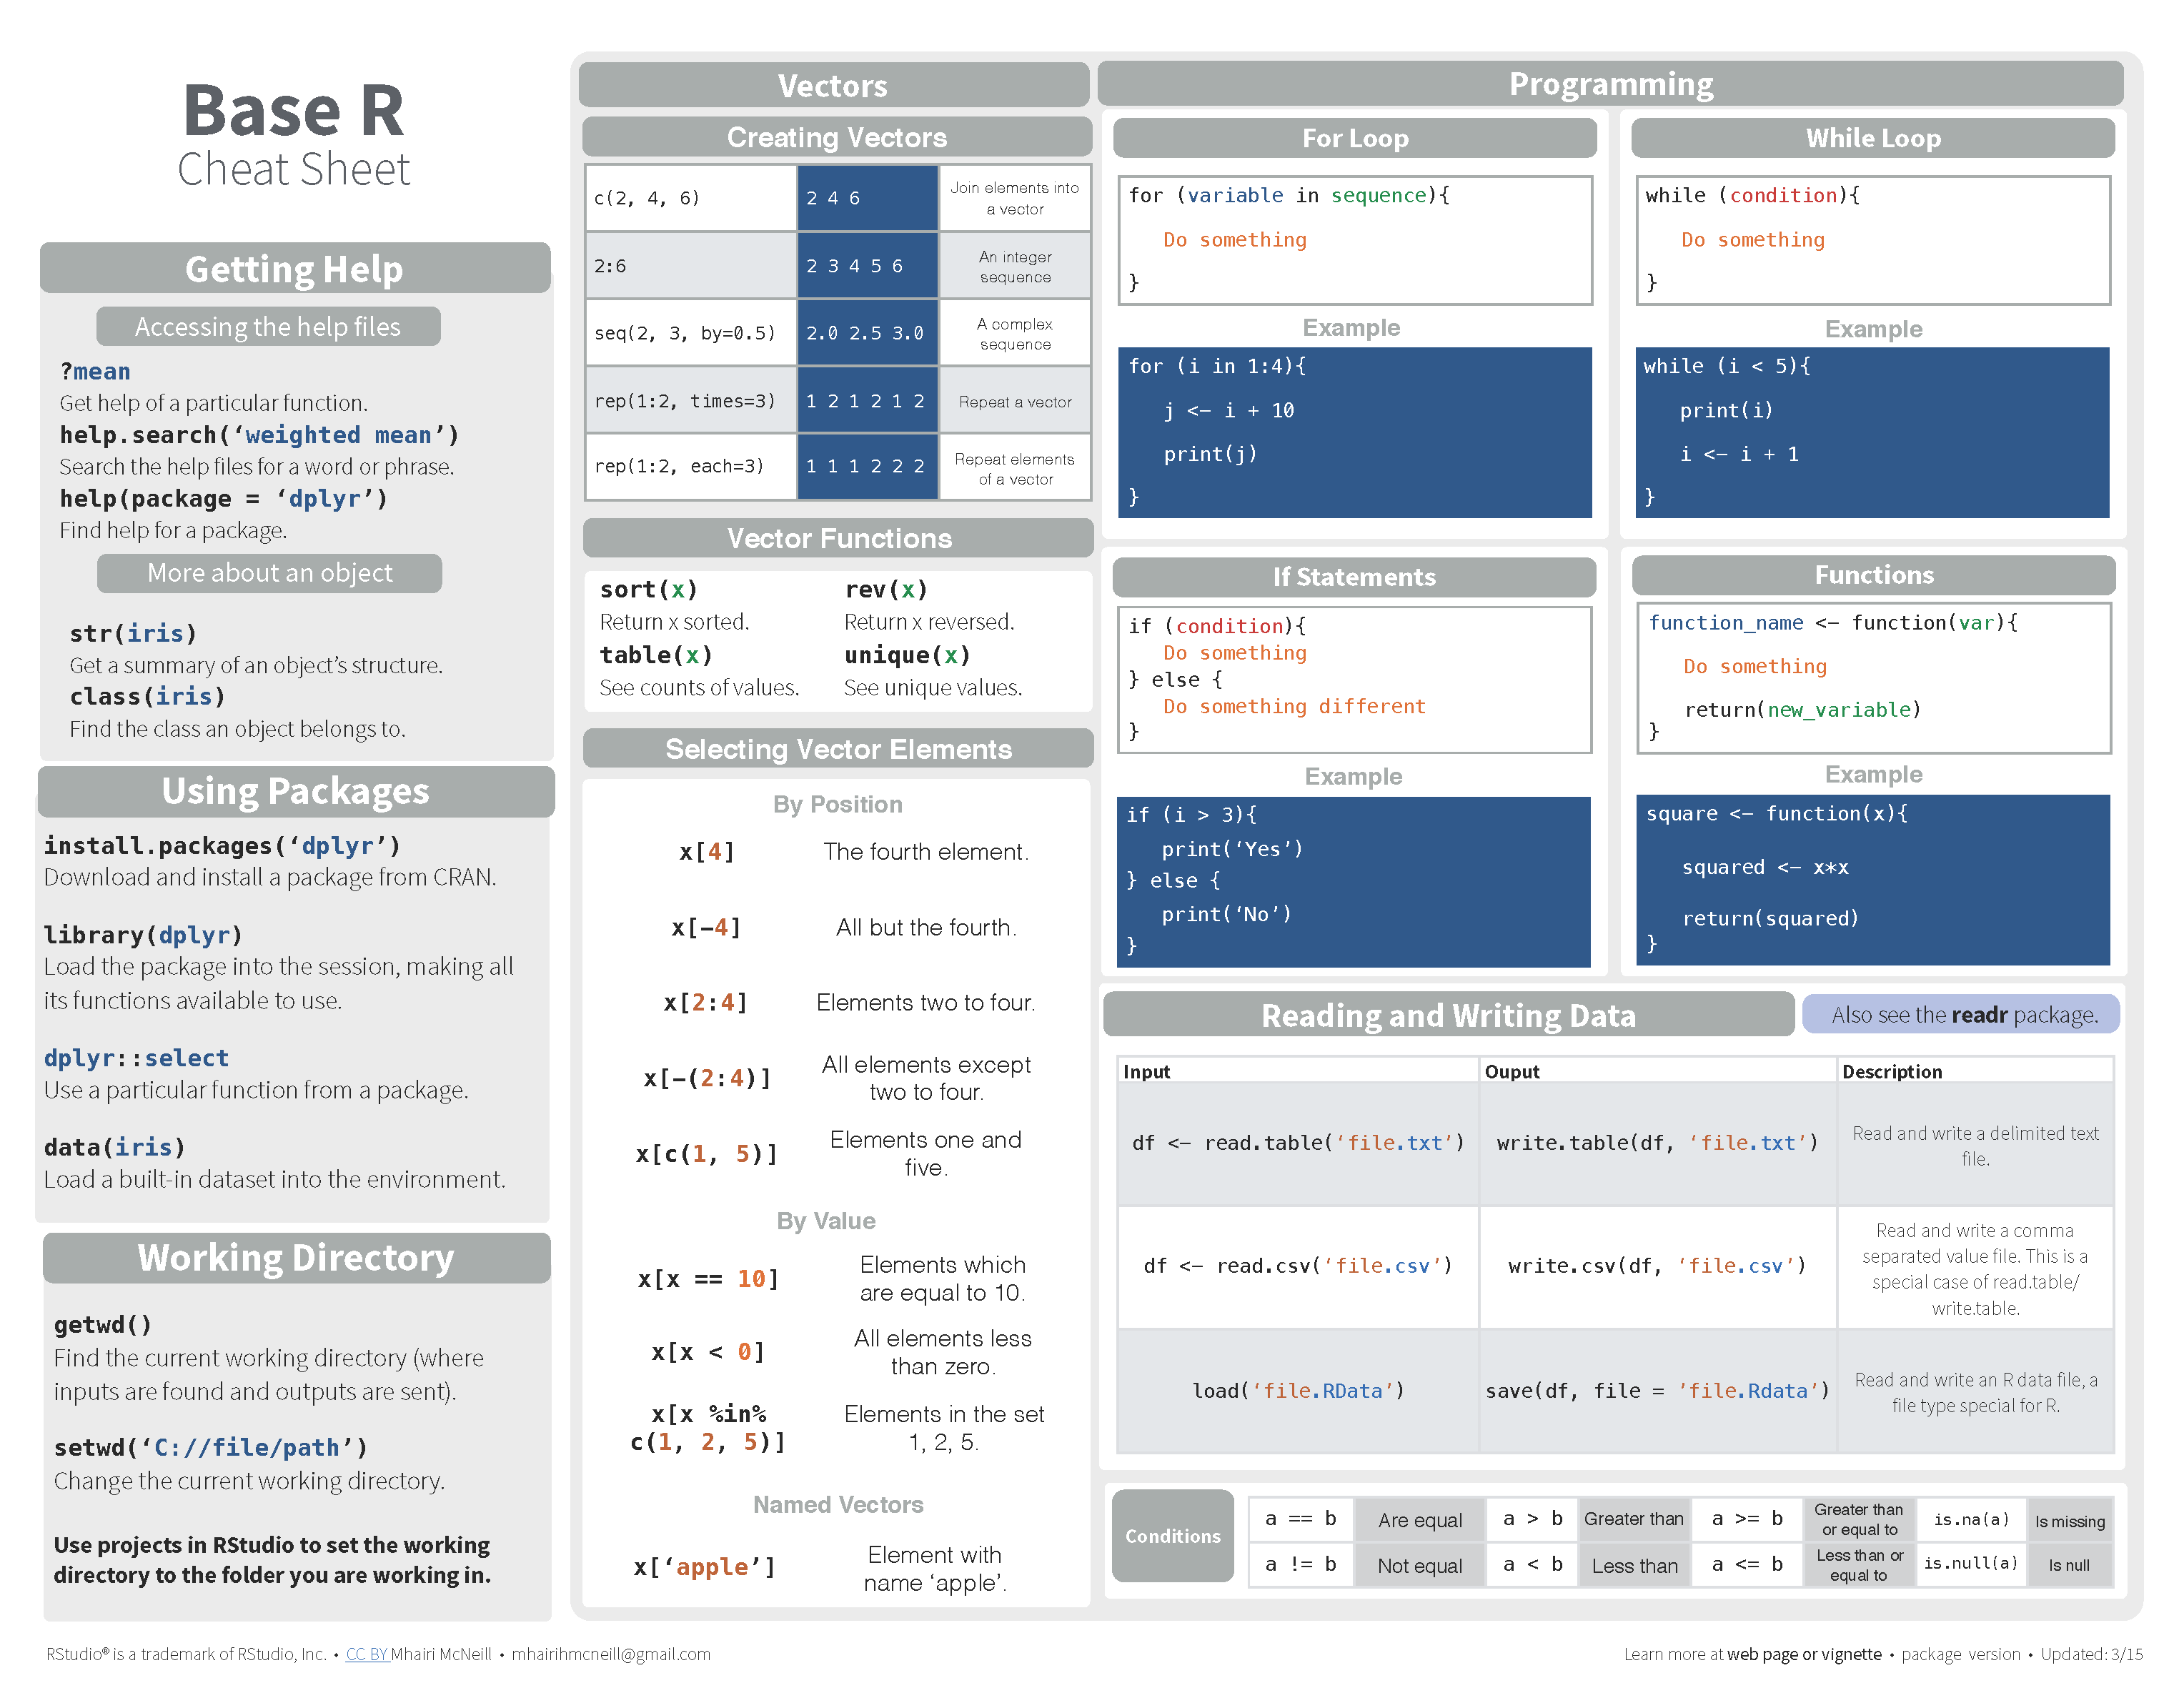
\includegraphics{images/base-r_1.png}
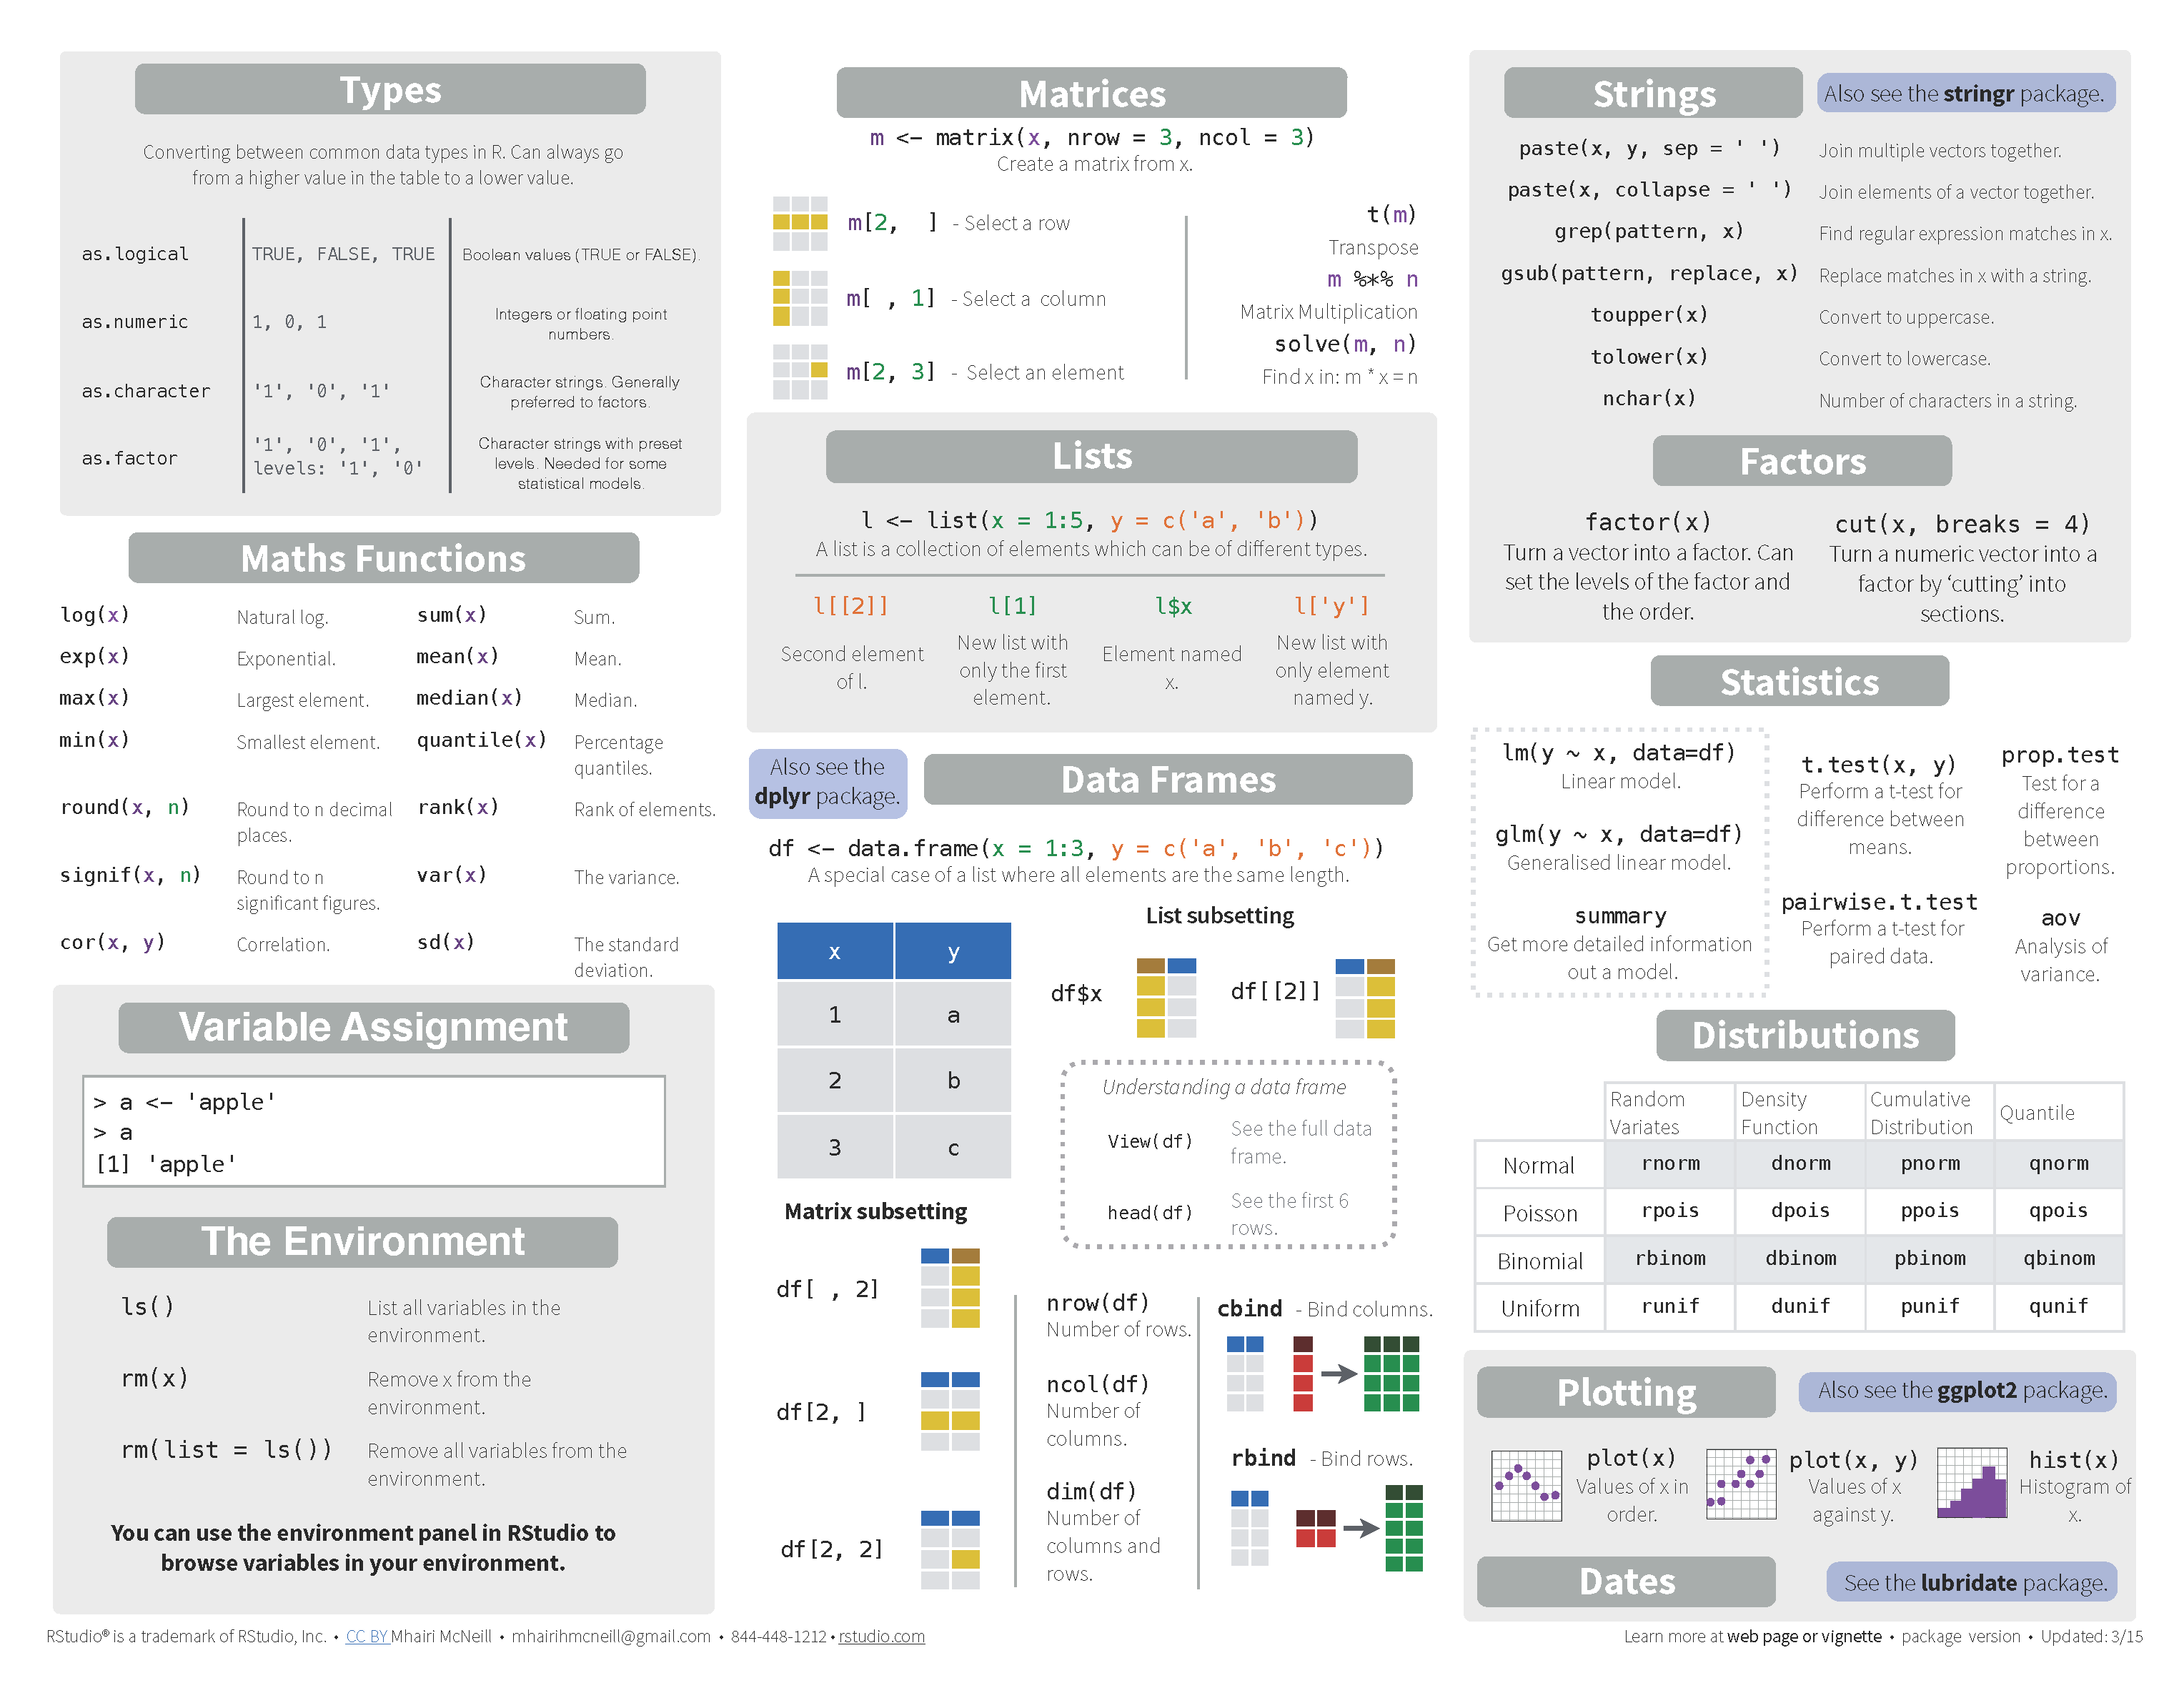
\includegraphics{images/base-r_2.png}

\bibliography{book.bib,packages.bib}


\end{document}
